\documentclass[11pt]{article}

\usepackage[utf8]{inputenc}
\usepackage[english]{babel}
\usepackage{courier}
\usepackage{graphicx}
\usepackage[bottom]{footmisc}
\usepackage{bytefield}
\usepackage{hyperref}
\usepackage{bookmark}
\usepackage{color}
\usepackage{alltt}
\usepackage{tabu, booktabs}

\title{DJ Link Packet Analysis}
\author{James Elliott\\Deep Symmetry, LLC}

\begin{document}

\maketitle

\abstract{The protocol used by Pioneer professional DJ equipment to
  communicate and coordinate performances can be monitored to provide
  useful information for synchronizing other software, such as light
  shows and sequencers. By creating a ``virtual CDJ'' that sends
  appropriate packets to the network, other devices can be induced to
  send packets containing even more useful information about their
  state. This article documents what has been learned so far about the
  protocol, and how to accomplish these tasks.}

\pagestyle{headings}

%% Define macros used to draw more complex message byte fields with
%% labeled headers and color-related sections.

\newcommand\hexhead{
  \bitbox[]{1}{\tiny\bfseries 0}
  \bitbox[]{1}{\tiny\bfseries 1}
  \bitbox[]{1}{\tiny\bfseries 2}
  \bitbox[]{1}{\tiny\bfseries 3}
  \bitbox[]{1}{\tiny\bfseries 4}
  \bitbox[]{1}{\tiny\bfseries 5}
  \bitbox[]{1}{\tiny\bfseries 6}
  \bitbox[]{1}{\tiny\bfseries 7}
  \bitbox[]{1}{\tiny\bfseries 8}
  \bitbox[]{1}{\tiny\bfseries 9}
  \bitbox[]{1}{\tiny\bfseries a}
  \bitbox[]{1}{\tiny\bfseries b}
  \bitbox[]{1}{\tiny\bfseries c}
  \bitbox[]{1}{\tiny\bfseries d}
  \bitbox[]{1}{\tiny\bfseries e}
  \bitbox[]{1}{\tiny\bfseries f}
}

\newcommand\messagehead{
  \bitbox[]{5}{\tiny\bfseries start}
  \bitbox[]{5}{\tiny $TxID$}
  \bitbox[]{3}{\tiny $type$}
  \bitbox[]{2}{\tiny $args$}
  \bitbox[]{1}{\tiny $tags$}
}

\newcommand{\baselinealign}[1]{%
  \centering
  \strut#1%
}

%%\newcommand{\colorbitbox}[4][rlbt]{%
%%    \rlap{\bitbox[#1]{#3}{\color{#2}\rule{\dimexpr\width-0.4pt}{\dimexpr\height-0.4pt}}}%
%%    \bitbox[#1]{#3}{#4}}

\newcommand{\colorbitbox}[4][rlbt]{%
  \sbox0{\bitbox[#1]{#3}{#4}}%
 \makebox[0pt][l]{\textcolor{#2}{\rule[-\dp0]{\wd0}{\ht0}}}%
 \bitbox[#1]{#3}{#4}%
}

%%\newcommand{\colorbitboxes*}[3]{%
%%  \sbox0{\bitboxes*{#2}{#3}}%
%%  \makebox[0pt][l]{\textcolor{#1}{\rule[-\dp0]{\wd0}{\ht0}}}%
%%  \bitboxes*{#2}{#3}%
%%}

\definecolor{lightgreen}{rgb}{0.64,1,0.71}
\definecolor{yellow}{rgb}{1,1,0.71}
\definecolor{lightred}{rgb}{1,0.7,0.71}
\definecolor{lightcyan}{rgb}{0.84,1,1}
\definecolor{lightpurple}{rgb}{1,0.71,1}

\tableofcontents

\newpage

\section{Mixer Startup}

When the mixer starts up, after it obtains an IP address (or gives up
on doing that and self-assigns an address), it sends out what look
like a series of packets\footnote{The packet capture described in this
  analysis can be found at
  \url{https://github.com/brunchboy/dysentery/raw/master/doc/assets/powerup.pcapng}}
simply announcing its existence to UDP port 50000 on the broadcast
address of the local network.

\begin{figure}
  \begin{bytefield}[bitwidth=1.5em,boxformatting={\baselinealign}]{16}
    \hexhead \\
    \begin{rightwordgroup}{Name}
      \begin{leftwordgroup}{Header}
        \bitboxes*{1}{{\tt 51} {\tt 73} {\tt 70} {\tt 74} {\tt 31} {\tt 57} {\tt 6d} {\tt 4a} {\tt 4f}
          {\tt 4c} {\tt \textbf{0a}} {\tt 00}}
        & \bitbox[lrt]{4}{}
      \end{leftwordgroup} \\
      \wordbox[lrb]{1}{Device Name (padded with {\tt 00})} 
    \end{rightwordgroup} \\
    \bitboxes*{1}{{\tt 01} {\tt 02} {\tt 00} {\tt 25} {\tt 02}}
  \end{bytefield}
  \caption{Initial announcement packets from Mixer}
  \label{fig:mixerInitial}
\end{figure}

These have a data length\footnote{Values within packets are shown in
  hexadecimal, while packet lengths and byte offsets are discussed in
  decimal.} of 37 bytes, appear roughly every 300 milliseconds, and
have the content shown in Figure~\ref{fig:mixerInitial}.

The tenth byte (inside what is labeled the header) is bolded because
its value changes in the different types of packets which follow.

After about three of these packets are sent, another series of three
begins. It is not clear what purpose these packets serve, because they
are not yet asserting ownership of any device number; perhaps they are
used when CDJs are powering up as part of the mechanism the mixer can
use to tell them which device number to use based on which network
port they are connected to?

\begin{figure}
  \begin{bytefield}[bitwidth=1.5em,boxformatting={\baselinealign}]{16}
    \hexhead \\
    \begin{rightwordgroup}{Name}
      \begin{leftwordgroup}{Header}
        \bitboxes*{1}{{\tt 51} {\tt 73} {\tt 70} {\tt 74} {\tt 31} {\tt 57} {\tt 6d} {\tt 4a} {\tt 4f}
          {\tt 4c} {\tt \textbf{00}} {\tt 00}}
        & \bitbox[lrt]{4}{}
      \end{leftwordgroup} \\
      \wordbox[lrb]{1}{Device Name (padded with {\tt 00})} 
    \end{rightwordgroup} \\
    \bitboxes*{1}{{\tt 01} {\tt 02} {\tt 00} {\tt 2c} {$N$} {\tt 02}} &
    \bitbox{6}{MAC address}
  \end{bytefield}
  \caption{First-stage Mixer device number assignment packets}
  \label{fig:mixerStage1}
\end{figure}

In any case, these three packets have a data length of 44 bytes, are
again sent to UDP port 50000 on the local network broadcast address,
at roughly 300 millisecond intervals, and have the content shown in
Figure~\ref{fig:mixerStage1}.

The value $N$ at byte~36 is 1, 2, or 3, depending on whether this
is the first, second, or third time the packet is sent.

After these comes another series of three numbered packets. These
appear to be claiming the device number for a particular device, as
well as announcing the IP address at which it can be found. They have
a data length of 50 bytes, and are again sent to UDP port 50000 on the
local network broadcast address, at roughly 300 millisecond intervals,
with the content shown in Figure~\ref{fig:mixerStage2}.

\begin{figure}[ht]
  \begin{bytefield}[bitwidth=1.5em,boxformatting={\baselinealign}]{16}
    \hexhead \\
    \begin{rightwordgroup}{Name}
      \begin{leftwordgroup}{Header}
        \bitboxes*{1}{{\tt 51} {\tt 73} {\tt 70} {\tt 74} {\tt 31} {\tt 57} {\tt 6d} {\tt 4a} {\tt 4f}
          {\tt 4c} {\tt \textbf{02}} {\tt 00}}
        & \bitbox[lrt]{4}{}
      \end{leftwordgroup} \\
      \wordbox[lrb]{1}{Device Name (padded with {\tt 00})} 
    \end{rightwordgroup} \\
    \bitboxes*{1}{{\tt 01} {\tt 02} {\tt 00} {\tt 32}} &
    \bitbox{4}{IP address} & \bitbox{6}{MAC address} &
    \bitbox{1}{$D$} & \bitbox{1}{$N$} \\
    \bitboxes*{1}{{\tt 02} {\tt 01}}
  \end{bytefield}
  \caption{Second-stage Mixer device number assignment packets}
  \label{fig:mixerStage2}
\end{figure}

I identify these as claiming/identifying the device number because the
value $D$ at byte~46 is the same as the device number that the
mixer uses to identify itself ({\tt 0x21}) and the same is true for the
corresponding packets seen from the CDJs (they use device numbers 2
and 3, as they are connected to those ports/channels on the mixer).

As with the previous series of three packets, the value $N$ at
byte~47 takes on the values 1, 2, and 3 in the three packets.

These are followed by another three packets, perhaps the last stage of
claiming the device number, again at 300 millisecond intervals, to the
same port 50000. These shorter packets have 38 bytes of data and the
content shown in Figure~\ref{fig:mixerStage3}.

\begin{figure}
  \begin{bytefield}[bitwidth=1.5em,boxformatting={\baselinealign}]{16}
    \hexhead \\
    \begin{rightwordgroup}{Name}
      \begin{leftwordgroup}{Header}
        \bitboxes*{1}{{\tt 51} {\tt 73} {\tt 70} {\tt 74} {\tt 31} {\tt 57} {\tt 6d} {\tt 4a} {\tt 4f}
          {\tt 4c} {\tt \textbf{04}} {\tt 00}}
        & \bitbox[lrt]{4}{}
      \end{leftwordgroup} \\
      \wordbox[lrb]{1}{Device Name (padded with {\tt 00})} 
    \end{rightwordgroup} \\
    \bitboxes*{1}{{\tt 01} {\tt 02} {\tt 00} {\tt 26}} &
    \bitbox{1}{$D$} & \bitbox{1}{$N$}
  \end{bytefield}
  \caption{Final-stage Mixer device number assignment packets}
  \label{fig:mixerStage3}
\end{figure}

As before the value $D$ at byte~36 is the same as the device
number that the mixer uses to identify itself ({\tt 0x21}) and
$N$ at byte~37 takes on the values 1, 2, and 3 in the three
packets.

Once those are sent, the mixer seems to settle down and send what
looks like a keep-alive packet to retain presence on the network and
ownership of its device number, at a less frequent interval. These
packets are 54 bytes long, again sent to port 50000 on the local
network broadcast address, roughly every second and a half. They have
the content shown in Figure~\ref{fig:mixerKeepalive}.

\begin{figure}[ht]
  \begin{bytefield}[bitwidth=1.5em,boxformatting={\baselinealign}]{16}
    \hexhead \\
    \begin{rightwordgroup}{Name}
      \begin{leftwordgroup}{Header}
        \bitboxes*{1}{{\tt 51} {\tt 73} {\tt 70} {\tt 74} {\tt 31} {\tt 57} {\tt 6d} {\tt 4a} {\tt 4f}
          {\tt 4c} {\tt \textbf{06}} {\tt 00}}
        & \bitbox[lrt]{4}{}
      \end{leftwordgroup} \\
      \wordbox[lrb]{1}{Device Name (padded with {\tt 00})} 
    \end{rightwordgroup} \\
    \bitboxes*{1}{{\tt 01} {\tt 02} {\tt 00} {\tt 36}} &
    \bitbox{1}{$D$} & \bitbox{1}{\tt 02} &
    \bitbox{6}{MAC address} & \bitbox{4}{IP address} \\
    \bitboxes*{1}{{\tt 01} {\tt 00} {\tt 00} {\tt 00} {\tt 02} {\tt 00}}
  \end{bytefield}
  \caption{Mixer keep-alive packets}
  \label{fig:mixerKeepalive}
\end{figure}

\section{CDJ Startup}

When a CDJ starts up the procedure and packets are nearly identical,
with groups of three packets sent at 300 millisecond intervals to port
50000 of the local network broadcast address. The only difference
between Figure~\ref{fig:cdjInitial} and Figure~\ref{fig:mixerInitial}
is the final byte, which is {\tt 0x01} for the CDJ, and was {\tt 0x02}
for the mixer.

\begin{figure}[ht]
  \begin{bytefield}[bitwidth=1.5em,boxformatting={\baselinealign}]{16}
    \hexhead \\
    \begin{rightwordgroup}{Name}
      \begin{leftwordgroup}{Header}
        \bitboxes*{1}{{\tt 51} {\tt 73} {\tt 70} {\tt 74} {\tt 31} {\tt 57} {\tt 6d} {\tt 4a} {\tt 4f}
          {\tt 4c} {\tt \textbf{0a}} {\tt 00}}
        & \bitbox[lrt]{4}{}
      \end{leftwordgroup} \\
      \wordbox[lrb]{1}{Device Name (padded with {\tt 00})} 
    \end{rightwordgroup} \\
    \bitboxes*{1}{{\tt 01} {\tt 02} {\tt 00} {\tt 25} {\tt 01}}
  \end{bytefield}
  \caption{Initial announcement packets from CDJ}
  \label{fig:cdjInitial}
\end{figure}

Similarly, the next series of three packets from the CDJ are nearly
identical to those from the mixer. The only difference between
Figure~\ref{fig:cdjStage1} and Figure~\ref{fig:mixerStage1} is byte~37
(immediately after the packet counter $N$), which again is {\tt 0x01}
for the CDJ, and was {\tt 0x02} for the mixer.

\begin{figure}
  \begin{bytefield}[bitwidth=1.5em,boxformatting={\baselinealign}]{16}
    \hexhead \\
    \begin{rightwordgroup}{Name}
      \begin{leftwordgroup}{Header}
        \bitboxes*{1}{{\tt 51} {\tt 73} {\tt 70} {\tt 74} {\tt 31} {\tt 57} {\tt 6d} {\tt 4a}
          {\tt 4f} {\tt 4c} {\tt \textbf{00}} {\tt 00}}
        & \bitbox[lrt]{4}{}
      \end{leftwordgroup} \\
      \wordbox[lrb]{1}{Device Name (padded with {\tt 00})} 
    \end{rightwordgroup} \\
    \bitboxes*{1}{{\tt 01} {\tt 02} {\tt 00} {\tt 2c} {$N$} {\tt 01}} &
    \bitbox{6}{MAC address}
  \end{bytefield}
  \caption{First-stage CDJ device number assignment packets}
  \label{fig:cdjStage1}
\end{figure}

However it appears that in this capture the CDJ skips the second stage
of claiming a device number, probably because it is configured to be
automatically assigned a device number based on the port of the mixer
to which it is connected, and we cannot see a packet that the mixer
sent it assigning it that device number. Instead, it jumps right to
the end of the third and final stage, sending a single 38-byte packet
with header byte~10 set to {tt 04} (which identified the three packets
of the third stage when the mixer was starting up), with content
identical to Figure~\ref{fig:mixerStage3}.

Even though the value of $N$ is {\tt 01}, this is the only packet
in this series that the CDJ sends. It would probably behave
differently if configured to assign its own device number (behaving
like we saw the mixer behave in claiming its device number).

The CDJ then moves to the keep-alive stage, sending out 54-byte
packets with the content shown in Figure~\ref{fig:cdjKeepalive}.

\begin{figure}[ht]
  \begin{bytefield}[bitwidth=1.5em,boxformatting={\baselinealign}]{16}
    \hexhead \\
    \begin{rightwordgroup}{Name}
      \begin{leftwordgroup}{Header}
        \bitboxes*{1}{{\tt 51} {\tt 73} {\tt 70} {\tt 74} {\tt 31} {\tt 57} {\tt 6d} {\tt 4a} {\tt 4f}
          {\tt 4c} {\tt \textbf{06}} {\tt 00}}
        & \bitbox[lrt]{4}{}
      \end{leftwordgroup} \\
      \wordbox[lrb]{1}{Device Name (padded with {\tt 00})} 
    \end{rightwordgroup} \\
    \bitboxes*{1}{{\tt 01} {\tt 02} {\tt 00} {\tt 36}} &
    \bitbox{1}{$D$} & \bitbox{1}{\tt 01} &
    \bitbox{6}{MAC address} & \bitbox{4}{IP address} \\
    \bitboxes*{1}{{\tt 01} {\tt 00} {\tt 00} {\tt 00} {\tt 01} {\tt 00}}
  \end{bytefield}
  \caption{CDJ keep-alive packets}
  \label{fig:cdjKeepalive}
\end{figure}

As seems to always be the case when comparing mixer and CDJ packets,
the difference between this and Figure~\ref{fig:mixerKeepalive} is
that byte~37 (following the device number $D$) has the value {\tt 01}
rather than {\tt 02}, and the same is true of the second-to-last byte
in each of the packets. (Byte~52 is {\tt 01} in
Figure~\ref{fig:cdjKeepalive} and {\tt 02} in
Figure~\ref{fig:mixerKeepalive}.

\section{Tracking BPM and Beats}
\label{sec:beatPackets}

For some time now,
Afterglow\footnote{\url{https://github.com/brunchboy/afterglow\#afterglow}}
has been able to synchronize its light shows with music being played
on Pioneer equipment by observing packets broadcast by the mixer to
port 50001. Until recently, however, it was not possible to tell which
player was the master, so there was no way to determine the down beat
(the start of each measure). Now that it is possible to to determine
which CDJ is the master player using the packets described in
Section~\ref{sec:virtualCdj}, these beat packets have become far more
useful, and Afterglow will soon be using them to track the down beat
based on the beat number reported by the master player.

To track beats, open a socket and bind it to port 50001. The devices
seem to broadcast two different kinds of packets to this port, a
shorter packet containing 45 bytes of data, and a longer packet
containing 96 bytes. The shorter packets seem to all have identical
content, and do not seem to convey useful information, so we currently
simply ignore them.

The 96-byte packets are sent on each beat, so even the arrival of the
packet is interesting information, it means that the player is
starting a new beat. (CDJs send these packets only when they are
playing \emph{and only for rekordbox-analyzed tracks}. The mixer sends
them all the time, acting as a backup metronome when no other device
is counting beats.) The content of these packets is shown in
Figure~\ref{fig:beatPacket}.

\begin{figure}
  \begin{bytefield}[bitwidth=1.9em, leftcurly=., leftcurlyspace=0pt, boxformatting={\baselinealign}]{16}
    \hexhead \\

    \begin{leftwordgroup}{\tiny\bfseries 00}
      \bitboxes*{1}{{\tt 51} {\tt 73} {\tt 70} {\tt 74} {\tt 31} {\tt 57} {\tt 6d} {\tt 4a} {\tt 4f}
        {\tt 4c} {\tt \textbf{28}}}
      & \bitbox[lrt]{5}{}
    \end{leftwordgroup} \\
    
    \begin{leftwordgroup}{\tiny\bfseries 10}
      \bitbox[lrb]{15}{Device Name (padded with {\tt 00})} \bitbox{1}{\tt 01}
    \end{leftwordgroup} \\
    
    \begin{leftwordgroup}{\tiny\bfseries 20}
      \bitbox{1}{\tt 00} & \bitbox{1}{$D$} & \bitboxes*{1}{{\tt 00} {\tt 3c}} &
      \bitbox{4}{$nextBeat$} & \bitbox{4}{$2ndBeat$} & \bitbox{4}{$nextBar$}
    \end{leftwordgroup} \\

    \begin{leftwordgroup}{\tiny\bfseries 30}
      \bitbox{4}{$4thBeat$} & \bitbox{4}{$2ndBar$} & \bitbox{4}{$8thBeat$} &
      \bitboxes*{1}{{\tt ff} {\tt ff} {\tt ff} {\tt ff}}
    \end{leftwordgroup} \\

    \begin{leftwordgroup}{\tiny\bfseries 40}
      \bitboxes*{1}{{\tt ff} {\tt ff} {\tt ff} {\tt ff} {\tt ff} {\tt ff} {\tt ff} {\tt ff}
        {\tt ff} {\tt ff} {\tt ff} {\tt ff} {\tt ff} {\tt ff} {\tt ff} {\tt ff}}
    \end{leftwordgroup} \\

    \begin{leftwordgroup}{\tiny\bfseries 50}
      \bitboxes*{1}{{\tt ff} {\tt ff} {\tt ff} {\tt ff}} & \bitbox{4}{$Pitch$} &
      \bitboxes*{1}{{\tt 00} {\tt 00}} & \bitbox{2}{$BPM$} & \bitbox{1}{$B_b$} & \bitboxes*{1}{{\tt 00} {\tt 00}} &
      \bitbox{1}{$D$}
    \end{leftwordgroup}

  \end{bytefield}
  \caption{Beat packets}
  \label{fig:beatPacket}
\end{figure}

The Device Number in $D$ (bytes~33 and 95) is the Player Number as
displayed on the CDJ itself, or 33 for the mixer, or another value for
a computer running rekordbox.

To facilitate synchronization of variable-tempo tracks, the number of
milliseconds after which a variety of upcoming beats will occur are
reported. $nextBeat$ at bytes~36--39 is the number of milliseconds in
which the very next beat will arrive. $2ndBeat$ (bytes~40--43) is the
number of milliseconds until the beat after that. $nextBar$
(bytes~44--47) reports the number of milliseconds until the next
measure of music begins, which may be from 1 to 4 beats away.
$4thBeat$ (bytes~48--51) reports how many millisecond will elapse
until the fourth upcoming beat; $2ndBar$ (bytes~52--55) the interval
until the second measure after the current one begins (which will
occur in 5 to 8 beats, depending how far into the current measure we
have reached); and $8thBeat$ (bytes~56--59) tells how many millieconds
we have to wait until the eighth upcoming beat will arrive.

The player's current pitch adjustment\footnote{The mixer always
  reports a pitch of $+0\%$.} can be found in bytes~84--87, labeled
$Pitch$. It represents a three-byte pitch adjustment percentage, where
{\tt 0x00100000} represents no adjustment ($0\%$), {\tt 0x00000000}
represents slowing all the way to a complete stop ($-100\%$, reachable
only in Wide tempo mode), and {\tt 0x00200000} represents playing at
double speed ($+100\%$).

The pitch adjustment percentage represented by $Pitch$ is calculated
as follows:

\begin{displaymath}
  100 \times
  \frac{(byte[85] \times 65536 + byte[86]  \times 256 + byte[87]) - 1048576}{1048576}
\end{displaymath}

The current BPM of the track playing on the device\footnote{The mixer
  passes along the BPM of the master player.} can be found at bytes~90--91
(labeled $BPM$). It is a two-byte integer representing one hundred
times the current track BPM. So, the current track BPM value to two
decimal places can be calculated as:

\[ \frac{byte[90] \times 256 + byte[91]}{100} \]

In order to obtain the actual playing BPM (the value shown in the BPM
display), this value must be multiplied by the current pitch
adjustment. Since calculating the effective BPM reported by a CDJ is a
common operation, here a simplified equation that results in the
effective BPM to two decimal places, by combinining the $BPM$ and
$Pitch$ values:\footnote{Since the mixer always reports a pitch
  adjustment of $+0\%$, its $BPM$ value can be used directly without
  this additional step.}

\[ \frac{(byte[90] \times 256 + byte[91]) \times (byte[85] \times 65536 + byte[86]  \times 256 + byte[87])}
   {104857600} \]

The counter $B_b$ at byte~92 counts out the beat within each bar,
cycling $1\to2\to3\to4$ repeatedly, and can be used to identify the
down beat if it is coming from the master player.

\section{Creating a Virtual CDJ}
\label{sec:virtualCdj}

Although some useful information can be obtained simply by watching
broadcast traffic on a network containing Pioneer gear, in order to
get important details it is necessary to cause the gear to send you
information directly. This can be done by simulating a ``Virtual
CDJ''.\footnote{Thanks are due to Diogo Santos for discovering the
  trick of creating a virtual CDJ in order to receive detailed status
  information from other devices.}

To do this, bind a UDP server socket to port 50002 on the network
interface on which you are receiving DJ-Link traffic, and start
sending keep-alive packets to port 50000 on the broadcast address as
if you were a CDJ. Follow the structure shown in
Figure~\ref{fig:cdjKeepalive}, but use the actual MAC and IP addresses
of the network interface on which you are receiving DJ-Link traffic,
so the devices can see how to reach you.

You can use a value like 5 for $D$ (the device/player number) so
as not to conflict with any actual players you have on the network,
and any name you would like. As long as you are sending these packets
roughly every 1.5 seconds, the other players and mixers will begin
sending packets directly to the socket you have opened on port 50002.

Each device seems to send status packets roughly every 200 milliseconds.

We are just beginning to analyze all the information which can be
gleaned from these packets, but here is what we know so
far.\footnote{Examples of packets discussed in this section can be
  found in the capture at
  \url{https://github.com/brunchboy/dysentery/raw/master/doc/assets/to-virtual.pcapng}}

\subsection{Mixer Status Packets}

Packets from the mixer will have a length of 56 bytes and the content
shown in Figure~\ref{fig:mixerStatus}.

\begin{figure}[h]
  \begin{bytefield}[bitwidth=1.9em, leftcurly=., leftcurlyspace=0pt, boxformatting={\baselinealign}]{16}
    \hexhead \\

    \begin{leftwordgroup}{\tiny\bfseries 00}
      \bitboxes*{1}{{\tt 51} {\tt 73} {\tt 70} {\tt 74} {\tt 31} {\tt 57} {\tt 6d} {\tt 4a} {\tt 4f}
        {\tt 4c} {\tt \textbf{29}}}
      & \bitbox[lrt]{5}{}
    \end{leftwordgroup} \\
    
    \begin{leftwordgroup}{\tiny\bfseries 10}
      \bitbox[lrb]{15}{Device Name (padded with {\tt 00})} \bitbox{1}{\tt 01}
    \end{leftwordgroup} \\
    
    \begin{leftwordgroup}{\tiny\bfseries 20}
      \bitbox{1}{\tt 00} & \bitbox{1}{$D$} & \bitboxes*{1}{{\tt 00} {\tt 14}} &
      \bitbox{1}{$D$} & \bitboxes*{1}{{\tt 00} {\tt 00}} & \bitbox{1}{$F$} &
      \bitboxes*{1}{{\tt 00} {\tt 10} {\tt 00} {\tt 00} {\tt 80} {\tt 00}} & \bitbox{2}{$BPM$}
    \end{leftwordgroup} \\
    
    \begin{leftwordgroup}{\tiny\bfseries 30}
      \bitboxes*{1}{{\tt 00} {\tt 10} {\tt 00} {\tt 00} {\tt 00} {\tt 09}} &
      \bitbox{1}{$X$} & \bitbox{1}{$B_b$} & \bitbox[]{8}{}
    \end{leftwordgroup}
  \end{bytefield}
  \caption{Mixer status packets}
  \label{fig:mixerStatus}
\end{figure}

Packets coming from a DJM-2000 nexus connected as the only mixer on
the network contain a value of 33 ({\tt 0x21}) for their Device Number
$D$ (bytes~33 and 36).

The value marked $F$ at byte~39 is evidently a status flag equivalent
to the one shown in Figure~\ref{fig:cdjStateFlags}, although on a
mixer the only two values seen so far are {\tt 0xf0} when it is the
tempo master, and {\tt 0xd0} when it is not. So evidently the mixer
always considers itself to be playing and synced, but never on-air.

There are two places that might contain pitch values, bytes~41--43 and
bytes~50--51, but since they always {\tt 0x100000} (or $+0\%$), we
can't be sure. The current tempo in beats-per-minute identified by the
mixer can be obtained as:

\[ \frac{byte[46] \times 256 + byte[47]}{100} \]

This value is labeled $BPM$ in Figure~\ref{fig:mixerStatus}.
Unfortunately, this BPM seems to only be valid when a
rekordbox-analyzed source is playing; when the mixer is doing its own
beat detection from unanalyzed audio sources, even though it displays
the detected BPM on the mixer itself, and uses that to drive its beat
effects, it does not send that value in these packets.

The current beat number within a bar (1, 2, 3 or 4) is sent in
$byte[55]$, labeled $B_b$. However, the beat number is \emph{not}
synchronized with the master player, and these packets do not arrive
at the same time as the beat started anyway, so this value is not
useful for much. The beat number should be determined, when needed,
from beat packets (described in Section~\ref{sec:beatPackets}) that
are sent by the master player.

The value at $byte[54]$, labeled $X$, has an unknown meaning. It
seems to start out with the value {\tt 0x00}, and then change when a
player starts playing to the value {\tt 0xff}, but it may well do
other things as well.

\subsection{CDJ Status Packets}

Packets from a CDJ will have a length of 212 bytes and the content
shown in Figure~\ref{fig:cdjStatus} for nexus players. Older players
send 208-byte packets with slightly less information. Newer firmware
and Nexus 2 players send packets that are 284 or 292~bytes long.

\begin{figure}
  \begin{bytefield}[bitwidth=1.9em, leftcurly=., leftcurlyspace=0pt, boxformatting={\baselinealign}]{16}
    \hexhead \\

    \begin{leftwordgroup}{\tiny\bfseries 00}
      \bitboxes*{1}{{\tt 51} {\tt 73} {\tt 70} {\tt 74} {\tt 31} {\tt 57} {\tt 6d} {\tt 4a} {\tt 4f}
        {\tt 4c} {\tt \textbf{0a}}}
      & \bitbox[lrt]{5}{}
    \end{leftwordgroup} \\
    
    \begin{leftwordgroup}{\tiny\bfseries 10}
      \bitbox[lrb]{15}{Device Name (padded with {\tt 00})} \bitbox{1}{\tt 01}
    \end{leftwordgroup} \\
    
    \begin{leftwordgroup}{\tiny\bfseries 20}
      \bitbox{1}{\tt 03} & \bitbox{1}{$D$} & \bitboxes*{1}{{\tt 00} {\tt b0}} &
      \bitbox{1}{$D$} & \bitboxes*{1}{{\tt 00} {\tt 01}} & \bitbox{1}{$A$} &
      \bitbox{1}{$D_r$} & \bitbox{1}{$S_r$} & \bitbox{1}{$t_r$} & \bitbox{1}{\tt 00} &
      \bitbox{4}{$rekordbox$}
    \end{leftwordgroup} \\

    \begin{leftwordgroup}{\tiny\bfseries 30}
      \bitboxes*{1}{{\tt 00} {\tt 00}} \bitbox{2}{$Track$} \bitboxes*{1}{{\tt 00} {\tt 00} {$t_2$} {$t_3$}
        {\tt 00} {\tt 00} {$t_4$} {$t_5$} {\tt 00} {\tt 00} {\tt 00} {\tt 00}}
    \end{leftwordgroup} \\

    \begin{leftwordgroup}{\tiny\bfseries 40}
      \bitboxes*{1}{{\tt 00} {\tt 00} {\tt 00} {\tt 00} {\tt 00} {\tt 00} {$t_6$} {$t_7$}
        {\tt 00} {\tt 00} {\tt 00} {\tt 00} {\tt 00} {\tt 00} {\tt 00} {\tt 00}}
    \end{leftwordgroup} \\

    \begin{leftwordgroup}{\tiny\bfseries 50}
      \bitboxes*{1}{{\tt 00} {\tt 00} {\tt 00} {\tt 00} {\tt 00} {\tt 00} {\tt 00} {\tt 00}
        {\tt 00} {\tt 00} {\tt 00} {\tt 00} {\tt 00} {\tt 00} {\tt 00} {\tt 00}}
    \end{leftwordgroup} \\

    \begin{leftwordgroup}{\tiny\bfseries 60}
      \bitboxes*{1}{{\tt 00} {\tt 00} {\tt 00} {\tt 00} {\tt 00} {\tt 00} {\tt 00} {\tt 00}
        {\tt 01} {\tt 00} {$U_a$} {$S_a$} {\tt 00} {\tt 00} {\tt 00} {$U_l$}}
    \end{leftwordgroup} \\

    \begin{leftwordgroup}{\tiny\bfseries 70}
      \bitboxes*{1}{{\tt 00} {\tt 00} {\tt 00} {$S_l$} {\tt 00}} & \bitbox{1}{$L$} & \bitboxes*{1}{{\tt 00} {\tt 00}
        {\tt 01} {\tt 00} {\tt 00}} & \bitbox{1}{$P_1$} & \bitbox{4}{$Firmware$}
    \end{leftwordgroup} \\

    \begin{leftwordgroup}{\tiny\bfseries 80}
      \bitboxes*{1}{{\tt 00} {\tt 00} {\tt 00} {\tt 00} {\tt 00} {\tt 00}} & \bitbox{2}{$Sync_n$} &
      \bitbox{1}{\tt 00} & \bitbox{1}{$F$} & \bitbox{1}{\tt ff} &
      \bitbox{1}{$P_2$} & \bitbox{4}{$Pitch_1$}
    \end{leftwordgroup} \\

    \begin{leftwordgroup}{\tiny\bfseries 90}
      \bitbox{2}{$l_1$} & \bitbox{2}{$BPM$} & \bitboxes*{1}{{\tt 7f} {\tt ff} {\tt ff} {\tt ff}} &
      \bitbox{4}{$Pitch_2$} & \bitbox{1}{\tt 00} & \bitbox{1}{$P_3$} & \bitbox{1}{\tt 00} & \bitbox{1}{\tt ff}
    \end{leftwordgroup} \\

    \begin{leftwordgroup}{\tiny\bfseries a0}
      \bitbox{4}{$Beat$} & \bitbox{2}{$Cue$} & \bitbox{1}{$B_b$} &
      \bitboxes*{1}{{\tt 00} {\tt 00} {\tt 00} {\tt 00} {\tt 00} {\tt 00} {\tt 00} {\tt 00} {\tt 00}}
    \end{leftwordgroup} \\

    \begin{leftwordgroup}{\tiny\bfseries b0}
      \bitboxes*{1}{{\tt 00} {\tt 00} {\tt 00} {\tt 00} {\tt 00} {\tt 00} {\tt 10} {\tt 00}
        {\tt 00} {\tt 00} {\tt 00} {\tt 00} {\tt 00} {\tt 00} {\tt 00} {\tt 00}}
    \end{leftwordgroup} \\

    \begin{leftwordgroup}{\tiny\bfseries c0}
      \bitbox{4}{$Pitch_3$} & \bitbox{4}{$Pitch_4$} &
      \bitbox{4}{$Packet$} & \bitbox{1}{$nx$} & \bitboxes*{1}{{\tt 00} {\tt 00} {\tt 00}}
    \end{leftwordgroup} \\

    \begin{leftwordgroup}{\tiny\bfseries d0}
      \bitboxes*{1}{{\tt 00} {\tt 00} {\tt 00} {\tt 00}} & \bitbox[]{12}{}
    \end{leftwordgroup}

  \end{bytefield}
  \caption{CDJ status packets}
  \label{fig:cdjStatus}
\end{figure}

The Device Number in $D$ (bytes~33 and 36) is the Player Number as
displayed on the CDJ itself. In the case of this capture, the CDJs
were assigned Player Numbers 2 and 3.

The activity flag $A$ at byte~39 seems to be 0 when the player is
idle, and 1 when it is playing, searching, or loading a track.

When a rekordbox track is loaded, the device holding the rekordbox
database from which the track was loaded is reported in $D_r$ at
byte~40 (if the track was loaded from the local device, this will be
the same as $D$; if it was loaded over the Link, it will be the number
of a different device) When no track is loaded, $D_r$ has the value
{\tt 00}.

Similarly, $S_r$ at byte~41 reports the slot from which the track was
loaded: The value {\tt 00} means no track is loaded, {\tt 01} means
the CD drive, {\tt 02} means the SD slot, and {\tt 03} means the USB
slot. When a track is loaded from a rekordbox collection on a laptop,
$S_r$ has the value {\tt 04}. $t_r$ at byte~42 may be an indicator of
whether the track came from rekordbox: It seems to have the value {\tt
  00} when no track is loaded or an unanalyzed track is loaded, {\tt
  01} when a rekordbox track is loaded, and {\tt 05} when an audio CD
is loaded.

The field $rekordbox$ at bytes~44--47 contains the rekordbox database
ID of the loaded track when a rekordbox track is being played.
Combined with the player number and slot information, this can be used
to request the track metadata as described in
Section~\ref{sec:metadata}. When an audio CD is loaded, this just
contains the track index on the disc.

The track number being played (its position within a playlist or other
scrolling list of tracks, as displayed on the CDJ) can be found at
bytes~50 and 51, labeled $Track$. (It may be a 4-byte value and also
include bytes~48 and 49, but that would seem an unmanageable number of
tracks to search through.)

There are a number of bytes, labeled $t_2$ through $t_7$, whose
purpose is as yet undetermined. They are all zero when there is no
track loaded, but take different values when a track is loaded.
(Actually, there are many other bytes than these which behave like
this, so they will probably be removed from the chart in a future
version of this document.)

Byte~106, labeled $U_a$ (for ``USB activity''), alternates between the
values 4 and 6 when there is USB activity---it may even alternate in
time with the flashing USB indicator LED on the player, although
visual inspection suggests there is not a perfect correlation.
Byte~107, $S_a$, is the same kind of activity indicator for the SD
slot. Byte~111 ($U_l$ for ``USB local'') has the value 4 when there is
no USB media loaded, 0 when USB is loaded, and 2 or 3 when the USB
Stop button has been pressed and the USB media is being unmounted.

Byte~115 ($S_l$ for ``SD local'') has the value 4 when there is no SD
media loaded, 0 when SD is loaded, and 2 or 3 when the SD door has
been opened and the SD media is being unmounted.

Byte~117, labeled $L$ (for ``Link available''), appears to have the
value 1 whenever USB, SD, or CD media is present in any player on the
network, whether or not the Link option is chosen in the other
players, and 0 otherwise.

\begin{samepage}
Byte~123, labeled $P_1$, appears to describe the current play mode.
The values seen so far, and their apparent meanings, are:

\begin{center}
  \begin{tabu}{rX}
    \toprule

    \bfseries{Value} & \bfseries{Meaning} \\

    0 & No track is loaded \\

    2 & A track is in the process of loading \\

    3 & Player is playing normally \\

    4 & Player is playing a loop \\

    5 & Player is paused anywhere other than the cue point \\

    6 & Player is paused at the cue point \\

    7 & Cue Play is in progress (playback while the cue button is
  held down) \\

  8 & Cue scratch is in progress \\

  9 & Player is searching forwards or backwards \\

  17 & Player reached the end of the track and stopped \\

    \bottomrule
  \end{tabu}
\end{center}
\end{samepage}

The $Firmware$ value at bytes~124--127 is an ASCII represenation of the
firmware version running in the player.

The value $Sync_n$ at bytes~134--135 seems to increment whenever the
player syncs to a new tempo master (another player or the mixer). I am
assuming it is just a 2-byte value, because I tried syncing 256 times
and saw the counter expand from byte~135 to include byte~134. It may
actually be a 4-byte value and also involve bytes~132 and 133, but I
wasn't going to try changing sync 65,536 times or more to find out.
Perhaps we could write software to test that someday by forcing tempo
master changes.

Byte~137, labeled $F$, is a bit field containing some very useful
state flags, detailed in Figure~\ref{fig:cdjStateFlags}.\footnote{We
  have not yet seen any other values for bits 0, 1, 2, or 7 in $F$, so
  we're unsure if they also carry meaning. If you ever find different
  values for them, please let us know by filing an Issue at
  \url{https://github.com/brunchboy/dysentery/issues}} It seems to
only be available on nexus players, and others always send 0 for this
byte?

\begin{figure}
  \begin{bytefield}[endianness=big,bitwidth=4em]{8}
    \bitheader{0-7} \\
    \bitbox{1}{\tt 1} & \bitbox{1}{\small{Play}} & \bitbox{1}{\small{Master}} & \bitbox{1}{\small{Sync}}
    \bitbox{1}{\small{On-Air}} & \bitbox{1}{\tt 1} & \bitbox{1}{\tt 0} & \bitbox{1}{\tt 0}
  \end{bytefield}
  \caption{CDJ state flag bits}
  \label{fig:cdjStateFlags}
\end{figure}

Byte~139, labeled $P_2$ seems to be another play state indicator,
having the value 122 ({\tt 0x7a}) when playing and 126 ({\tt 0x7e})
when stopped. When the CDJ is trying to play, but is being held in
place by the DJ holding down on the jog wheel, $P_1$ considers it to
be playing (value 3), while $P_2$ considers it to be stopped (value
126). Non-nexus players seem to use the value 106 ({\tt 0x6a}) when
playing and 110 ({\tt 0x6e}) when stopped, while nxs2 players use the
values 250 and 254 ({\tt 0xfa} and {\tt 0xfe}) so this seems to be
another bit field like $F$.

There are four different places where pitch information appears in
these packets: $Pitch_1$ at bytes~141--143, $Pitch_2$ at
bytes~153--155, $Pitch_3$ at bytes~193--195, and $Pitch_4$ at
bytes~197--199.

Each of these values represents a three-byte pitch adjustment
percentage, where {\tt 0x100000} represents no adjustment ($0\%$),
{\tt 0x000000} represents slowing all the way to a complete stop
($-100\%$, reachable only in Wide tempo mode), and {\tt 0x200000}
represents playing at double speed ($+100\%$).

Note that if playback is stopped by pushing the pitch fader all the
way to $-100\%$ in Wide mode, both $P_1$ and $P_2$ still show it as
playing, which is different than when the jog wheel is held down,
since $P_2$ shows a stop in the latter situation.

Here is how the pitch adjustment percentage represented by $Pitch_1$
would be calculated:

\begin{displaymath}
  100 \times
  \frac{(byte[141] \times 65536 + byte[142]  \times 256 + byte[143]) - 1048576}{1048576}
\end{displaymath}

We don't know why there are so many copies of the pitch information,
or all circumstances under which they might differ from each other,
but it seems that $Pitch_1$ and $Pitch_3$ report the current pitch
adjustment actually in effect (as reflected on the BPM display),
whether it is due to the local pitch fader, or a synced tempo master.

$Pitch_2$ and $Pitch_4$ are always tied to the position of the local
pitch fader, unless Tempo Reset is active, effectively locking the
pitch fader to 0\% and $Pitch_2$ and $Pitch_4$ to {\tt 0x100000}, or
the player is paused or the jog wheel is being held down, freezing
playback and locking the local pitch to $-100\%$, in which case they
both have the value {\tt 0x000000}.

When playback stops, either due to the play button being pressed or
the jog wheel held down, the value of $Pitch_4$ drops to {\tt
  0x000000} instantly, while the value of $Pitch_2$ drops over time,
reflecting the gradual slowdown of playback which is controlled by the
player's brake speed setting. When playback starts, again either due
to the play button being pressed or the jog wheel being released, both
$Pitch_2$ and $Pitch_4$ gradually rise to the target pitch, at a speed
controlled by the player's release speed setting.

If the player is \emph{not} synced, but the current pitch is different
than what the pitch fader would indicate (in other words, the player
is in the mode where it tells you to move the pitch fader to the
current BPM in order to change the pitch), moving the pitch fader
changes the values of $Pitch_2$ and $Pitch_4$ until they match
$Pitch_1$ and $Pitch_3$ and begin to affect the actual effective
pitch. From that point on, moving the pitch fader sets the value of
all of $Pitch_1$, $Pitch_2$, $Pitch_3$, and $Pitch_4$. This all seems
more complicated than it really needs to be...

The current BPM of the track (the BPM at the point that is currently
being played, or at the location where the player is currently paused)
can be found at bytes~146--147 (labeled $BPM$). It is a two-byte
integer representing one hundred times the current track BPM. So, the
current track BPM value to two decimal places can be calculated as:

\[ \frac{byte[146] \times 256 + byte[147]}{100} \]

In order to obtain the actual playing BPM (the value shown in the BPM
display), this value must be multiplied by the current effective
pitch, calculated from $Pitch_1$ as described above. Since calculating
the effective BPM reported by a CDJ is a common operation, here a
simplified equation that results in the effective BPM to two decimal
places, by combinining the $BPM$ and $Pitch1$ values:

\[ \frac{(b[146] \times 256 + b[147]) \times (b[141] \times 65536 + b[142]  \times 256 + b[143])}
     {104857600} \]

Because Rekordbox and the CDJs support tracks with variable BPM, this
value can and does change over the course of playing such tracks. When
no track is loaded, $BPM$ has the value {\tt 0xffff}.

The meaning of value $l_1$ (bytes~144--145) is not currently known. It
may simply reflect whether a track is loaded or not: it seems to have
the value {\tt 0x7fff} when no track is loaded, {\tt 0x8000} when a
rekordbox track is loaded, and {\tt 0x0000} when a non-rekordbox track
(like from a physical CD) is loaded.

Byte~157 (labeled $P_3$) seems to communicate additional information
about the current play mode, with the following meanings that we have
found so far:
\begin{center}
  \begin{tabu}{rX}
    \toprule

    \bfseries{Value} & \bfseries{Meaning} \\

    0 & No track is loaded \\

    1 & Player is paused or playing in Reverse mode \\

    9 & Player is playing in Forward mode with jog mode set to Vinyl \\

    13 & Player is playing in Forward mode with jog mode set to CDJ \\

    \bottomrule
  \end{tabu}
\end{center}

The 4-byte beat counter (which counts each beat from 1 through the end
of the track) is found in bytes~160--163, labeled $Beat$. When the
player is paused at the start of the track, this seems to hold the
value 0, even though it is beat 1, and when no rekordbox-analyzed
track is loaded, \emph{and in packets from non-nexus players}, this
holds the value {\tt 0xffffffff}.

The counter $B_b$ at byte~166 counts out the beat within each bar,
cycling $1\to2\to3\to4$ repeatedly, and can be used to identify the
down beat (as is used in the Master Player display on the CDJs as a
mixing aid). Again, when no reckordbox-analyzed track is loaded, this
holds the value~0. If you want to synchronize events to the down beat,
use the CDJ status packets' $F$ value to identify the master player,
but use the beat packets sent by that player (described in
Section~\ref{sec:beatPackets}) to determine when the beats are
actually happening.

A countdown timer to the next saved cue point is available in
bytes~164--165 (labeled $Cue$). If there is no saved cue point after
the current play location in the track, or if it is further than 64
bars ahead, these bytes contain the value {\tt 0x01ff} and the CDJ
displays ``-\,-.-~bars''. As soon as there are just 64 bars (256
beats) to go before the next cue point, this value becomes {\tt
  0x0100}. This is the point at which the CDJ starts to display a
countdown, which it displays as ``63.4~bars''. As each beat goes by,
this value decreases by 1, until the cue point is about to be reached,
at which point the value is {\tt 0x0001} and the CDJ displays
``00.1~bars''. On the beat on which the cue point was saved the value
is {\tt 0x0000} and the CDJ displays ``00.0~Bars''. On the next beat,
the value becomes determined by the next cue point (if any) in the
track.

Bytes~200-203 seem to contain a 4-byte packet counter labeled
$Packet$, which is incremented for each packet sent by the player. (I
am just guessing it is four bytes long, I have not yet watched long
enough for the count to need more than the last three bytes).

Byte~204, labeled $nx$, seems to have the value {\tt 0x0f} for nexus
players, and {\tt 0x05} for older players.

\subsection{Rekordbox Status Packets}

Rekordbox sends status packets which appear to be essentially
identical to those sent by a mixer, as shown in
Figure~\ref{fig:mixerStatus}, sending ``rekordbox'' as its device
name. The device number $D$ (bytes~33 and 36) seems to be 41 ({\tt
  0x29}), although it will probably use conflict resolution to pick an
unused number if multiple copies are running. The $F$ value we have
seen remains consistent as a status flag, showing {\tt 0xc0} which
would indicate that it is always ``playing'' but not synced, tempo
master, nor on the air. The $BPM$ value seems to track that of the
master player, and the same potential pitch values (fixed at {\tt
  0x100000}, or +0\%) are present, as is $X$. $B_b$ always seems to be
zero.

\section{Track Metadata}
\label{sec:metadata}

Thanks to
@EvanPurkhiser\footnote{\url{https://github.com/EvanPurkhiser}}, we
finally started making progress in retrieving metadata from CDJs, and
now some shared code from Austin
Wright\footnote{\url{https://bitbucket.org/awwright/libpdjl}} is
boosting our understanding considerably!

To be polite about it, the first step is to determine the port on
which the player is offering its remote database server. That can be
determined by opening a TCP connection to port $12,523$ on the player
and sending it sending a packet with the content shown in
Figure~\ref{fig:dbServerQueryPacket}.

\begin{figure}
  \begin{bytefield}[bitwidth=1.9em, leftcurly=., leftcurlyspace=0pt, boxformatting={\baselinealign}]{16}
    \hexhead \\

    \begin{leftwordgroup}{\tiny\bfseries 00}
      \bitboxes*{1}{{\tt 00} {\tt 00} {\tt 00} {\tt 0f} {\tt R} {\tt e} {\tt m} {\tt o}
        {\tt t} {\tt e} {\tt D} {\tt B} {\tt S} {\tt e} {\tt r} {\tt v}}
    \end{leftwordgroup} \\
    
    \begin{leftwordgroup}{\tiny\bfseries 10}
      \bitboxes*{1}{{\tt e} {\tt r} {\tt 00}} & \bitbox[]{13}{}
    \end{leftwordgroup}
    
  \end{bytefield}
  \caption{DB Server query packet}
  \label{fig:dbServerQueryPacket}
\end{figure}

The player will send back a two-byte response, containing the high
byte of the port number followed by the low byte. So far, the response
from a CDJ has always indicated a port number of 1051, but using this
query to determine the port to use will protect you against any future
changes. The same query can also be sent to a laptop running rekordbox
to find the rekordbox database server port, which can also be queried
for metadata in the exact same way described below.

To find the metadata associated with a particular track, given its
rekordbox ID number, as well as the player and slot from which it was
loaded (all of which can be determined from a CDJ status packet
received by a virtual CDJ as described in
Section~\ref{sec:virtualCdj}), open a TCP connection to the device
from which the track was loaded, using the port that it gave you in
response to the DB Server query packet, then send the following four
packets.

The first packet sent to the database server contains the five bytes
{\tt 11 00 00 00 01}, and results in the same five bytes being sent
back.

All further packets have a shared structure. They consist of lists of
type-tagged fields (a type byte, followed some number of value bytes,
although in the case of the variable-size types, the first four bytes
are a big-endian integer that specifies the length of the additional
value bytes that make up the field). So far, there are four known
field types, and it turns out that the packet we just saw is one of
them, it represents the number 1 as a 4-byte integer.

\subsection{Field Types}

The first byte of a field identifies what type of field is coming. The
values {\tt 0x0f}, {\tt 0x10}, and {\tt 0x11} are followed by 1, 2,
and 4~byte fixed-length integer fields, while {\tt 0x14} and {\tt
  0x26} introduce variable-length fields, a binary blob and a UTF-16
big-endian string respectively.

\subsubsection{Number Fields}

Number fields are indicated by an initial byte~{\tt 0x0f}, {\tt 0x10},
or {\tt 0x11} which is followed by big-endian integer value of length
1, 2, or 4~bytes respectively, as shown in Figure~\ref{fig:numFields}.
So, as noted above, the initial greeting packet sent to and received
back from the database server is a number field, four bytes long,
representing the value 1.

\begin{figure}
  \begin{center}
    \begin{bytefield}[bitwidth=2em]{2}
      \bitheader{0-1} \\
      \bitbox{1}{\tt 0f}\bitbox{1}{$n$} \\
    \end{bytefield}

    \begin{bytefield}[bitwidth=2em]{3}
      \bitheader{0-2} \\
      \bitbox{1}{\tt 10}\bitbox{2}{$n$} \\
    \end{bytefield}

    \begin{bytefield}[bitwidth=2em]{5}
      \bitheader{0-4} \\
      \bitbox{1}{\tt 11}\bitbox{4}{$n$}
    \end{bytefield}
  \end{center}
  \caption{Number Fields of length 1, 2, and 4}
  \label{fig:numFields}
\end{figure}


\subsubsection{Binary Fields}

Variable-length binary (blob) fields are indicated by an initial
byte~{\tt 0x14}, followed by a 4~byte big-endian integer which
specifies the length of the field payload. The length is followed by
the specified number of bytes (for example, an album art image,
waveform or beat grid). This is illustrated in
Figure~\ref{fig:blobField}.

\begin{figure}
  \begin{bytefield}[bitwidth=1.9em, leftcurly=., leftcurlyspace=0pt, boxformatting={\baselinealign}]{16}
    \hexhead \\

    \bitbox{1}{\tt 14} & \bitbox{4}{$length$} & \bitbox[lrt]{11}{Binary data} \\
    \skippedwords \\
    \wordbox[lrb]{1}{}

  \end{bytefield}
  \caption{Binary (Blob) Field}
  \label{fig:blobField}
\end{figure}

\subsubsection{String Fields}

Variable-length string fields are indicated by an initial byte~{\tt
  0x26}, followed by a 4~byte big-endian integer which specifies the
length of the string, in two-byte UTF-16 big-endian characters. So the
length is folowed by $2 \times length$ bytes containing the actual
string characters. The last character of the string is always NUL,
represented by {\tt 0x0000}. This is illustrated in
Figure~\ref{fig:stringField}.

\begin{figure}
  \begin{bytefield}[bitwidth=1.9em, leftcurly=., leftcurlyspace=0pt, boxformatting={\baselinealign}]{16}
    \hexhead \\

    \bitbox{1}{\tt 26} & \bitbox{4}{$length$} & \bitbox[lrt]{11}{UTF-16BE string} \\
    \skippedwords \\
    \wordbox[lrb]{1}{}

  \end{bytefield}
  \caption{String Field}
  \label{fig:stringField}
\end{figure}

\subsection{Messages}
\label{sec:dbServerMessages}

Messages are introduced by a 4~byte Number field containing the magic
value {\tt 0x872349ae}. This is followed by another 4~byte number
field that contains a transaction ID, which starts at 1 and is
incremented for each query sent, and all messages sent in response to
that query will contain the same transaction ID. This is followed by a
2~byte number field containing the message type, a 1~byte number field
containing the number of argument fields present in the message, and a
blob field containing a series of bytes which identify the types of
each argument field. This blob is always 12~bytes long, regardless of
how few arguments there are (and presumably this means no message ever
has more than 12 arguments). Tag bytes past the actual argument count
of the message are set to 0.

The argument type tags use different values than the field type tags
themselves, for some reason, and it is not clear why this redundant
information is necessary at all, but that is true a number of places
in the protocol as you will see later. Here are the known tag values
and their meanings:

\begin{center}
  \begin{tabu}{rX}
    \toprule

    \bfseries{Tag} & \bfseries{Meaning} \\

    {\tt 0x02} & A string in UTF-16 big-endian encoding, with trailing
    NUL (zero) character \\

    {\tt 0x03} & A binary blob \\

    {\tt 0x06} & A 4~byte big-endian integer \\
    \bottomrule
  \end{tabu}
\end{center}

I am guessing that if we ever see them, a tag of 4 would represent a
1~byte integer, and 5 would represent a 2~byte integer. But so far no
such messages have been seen.

This header is followed by the fields that make up the message
arguments, if any. The header structure is illustrated in
Figure~\ref{fig:messageHeader}, where $TxID$ is the transaction ID,
$n$ is the number of arguments found in the message, and $t_1$ through
$t_{12}$ are the type tags for each argument, or 0 if there is no
argument in that position.

\begin{figure}
  \begin{bytefield}[bitwidth=1.9em, leftcurly=., leftcurlyspace=0pt, boxformatting={\baselinealign}]{16}
    \hexhead \\

    \begin{leftwordgroup}{\tiny\bfseries 00}
      
      \colorbitbox{lightgreen}{1}{\tt 11} & \colorbitbox{lightgreen}{4}{\tt 872349ae} &
      \colorbitbox{yellow}{1}{\tt 11} & \colorbitbox{yellow}{4}{$TxID$} &
      \colorbitbox{lightred}{1}{\tt 10} & \colorbitbox{lightred}{2}{$type$} &
      \colorbitbox{lightcyan}{1}{\tt 0f} & \colorbitbox{lightcyan}{1}{$n$} &
      \colorbitbox{lightpurple}{1}{\tt 14}
    \end{leftwordgroup} \\
    
    \begin{leftwordgroup}{\tiny\bfseries 10}
      \colorbitbox{lightpurple}{4}{{\tt 0000000c}\small{ (12)}} &
      \colorbitbox[lbt]{lightpurple}{1}{$t_1$} & \colorbitbox[bt]{lightpurple}{1}{$t_2$} &
      \colorbitbox[bt]{lightpurple}{1}{$t_3$} & \colorbitbox[bt]{lightpurple}{1}{$t_4$} &
      \colorbitbox[bt]{lightpurple}{1}{$t_5$} & \colorbitbox[bt]{lightpurple}{1}{$t_6$} &
      \colorbitbox[bt]{lightpurple}{1}{$t_7$} & \colorbitbox[bt]{lightpurple}{1}{$t_8$} &
      \colorbitbox[bt]{lightpurple}{1}{$t_9$} & \colorbitbox[bt]{lightpurple}{1}{$t_{10}$} &
      \colorbitbox[bt]{lightpurple}{1}{$t_{11}$} & \colorbitbox[rbt]{lightpurple}{1}{$t_{12}$}
    \end{leftwordgroup} \\

    \begin{leftwordgroup}{}
      \wordbox[lrt]{1}{Arguments} \\
      \skippedwords \\
      \wordbox[lrb]{1}{}
    \end{leftwordgroup}

  \end{bytefield}
  \caption{Message Header}
  \label{fig:messageHeader}
\end{figure}

Before you can send your first actual query, you need to send a
special message which seems to be necessary for establishing the
context for queries. It has a $type$ of 0, a special $TxID$ value of
{\tt 0xfffffffe}, and a single numeric argument, as shown in
Figure~\ref{fig:querySetupPacket}.

The value $D$ is, like in the other packets we have seen, a player
device number. In this case it is the device that is asking for
metadata information. It must be a valid player number between 1 and
4, and that player must actually be present on the network, must not
be the same player that you are contacting to request metadata from,
and must not be a player that has connected to that player via Link
and loaded a track from it. So the safest device number to use is the
device number you are using for your virtual CDJ, but since it must be
between 1 and 4, you can only do that if there are fewer than four
actual CDJs on the network.

\begin{figure}
  \begin{bytefield}[bitwidth=1.9em, leftcurly=., leftcurlyspace=0pt, boxformatting={\baselinealign}]{16}
    \hexhead \\
    \messagehead \\

    \begin{leftwordgroup}{\tiny\bfseries 00}

      \colorbitbox{lightgreen}{1}{\tt 11} & \colorbitbox{lightgreen}{4}{\tt 872349ae} &
      \colorbitbox{yellow}{1}{\tt 11} & \colorbitbox{yellow}{4}{\tt fffffffe} &
      \colorbitbox{lightred}{1}{\tt 10} & \colorbitbox{lightred}{2}{\tt 0000} &
      \colorbitbox{lightcyan}{1}{\tt 0f} & \colorbitbox{lightcyan}{1}{\tt 01} &
      \colorbitbox{lightpurple}{1}{\tt 14}
    \end{leftwordgroup} \\

    \begin{leftwordgroup}{\tiny\bfseries 10}
      \colorbitbox{lightpurple}{4}{{\tt 0000000c}\small{ (12)}} &
      \colorbitbox[lbt]{lightpurple}{1}{\tt 06} & \colorbitbox[bt]{lightpurple}{1}{\tt 00} &
      \colorbitbox[bt]{lightpurple}{1}{\tt 00} & \colorbitbox[bt]{lightpurple}{1}{\tt 00} &
      \colorbitbox[bt]{lightpurple}{1}{\tt 00} & \colorbitbox[bt]{lightpurple}{1}{\tt 00} &
      \colorbitbox[bt]{lightpurple}{1}{\tt 00} & \colorbitbox[bt]{lightpurple}{1}{\tt 00} &
      \colorbitbox[bt]{lightpurple}{1}{\tt 00} & \colorbitbox[bt]{lightpurple}{1}{\tt 00} &
      \colorbitbox[bt]{lightpurple}{1}{\tt 00} & \colorbitbox[rbt]{lightpurple}{1}{\tt 00}
    \end{leftwordgroup} \\

    \begin{leftwordgroup}{\tiny\bfseries 20}
      \bitbox{1}{\tt 11} & \bitbox{4}{$D_{ours}$} & \bitbox[]{11}{}
    \end{leftwordgroup}
    
  \end{bytefield}
  \caption{Query context setup message}
  \label{fig:querySetupPacket}
\end{figure}


The player will respond with a message of type {\tt 0x4000}, which is
the common ``success'' response when requested data is available. The
response message has two numeric arguments, the first of which is the
message type of the request we sent (which was 0), and the second
usually tells you the number of items that are available in response
to the query you made, but in this special setup query, it returns its
own player number. The overall structure is illustrated in
Figure~\ref{fig:querySetupResponse}.

\begin{figure}
  \begin{bytefield}[bitwidth=1.9em, leftcurly=., leftcurlyspace=0pt, boxformatting={\baselinealign}]{16}
    \hexhead \\
    \messagehead \\

    \begin{leftwordgroup}{\tiny\bfseries 00}

      \colorbitbox{lightgreen}{1}{\tt 11} & \colorbitbox{lightgreen}{4}{\tt 872349ae} &
      \colorbitbox{yellow}{1}{\tt 11} & \colorbitbox{yellow}{4}{\tt fffffffe} &
      \colorbitbox{lightred}{1}{\tt 10} & \colorbitbox{lightred}{2}{\tt 4000} &
      \colorbitbox{lightcyan}{1}{\tt 0f} & \colorbitbox{lightcyan}{1}{\tt 02} &
      \colorbitbox{lightpurple}{1}{\tt 14}
    \end{leftwordgroup} \\

    \begin{leftwordgroup}{\tiny\bfseries 10}
      \colorbitbox{lightpurple}{4}{{\tt 0000000c}\small{ (12)}} &
      \colorbitbox[lbt]{lightpurple}{1}{\tt 06} & \colorbitbox[bt]{lightpurple}{1}{\tt 06} &
      \colorbitbox[bt]{lightpurple}{1}{\tt 00} & \colorbitbox[bt]{lightpurple}{1}{\tt 00} &
      \colorbitbox[bt]{lightpurple}{1}{\tt 00} & \colorbitbox[bt]{lightpurple}{1}{\tt 00} &
      \colorbitbox[bt]{lightpurple}{1}{\tt 00} & \colorbitbox[bt]{lightpurple}{1}{\tt 00} &
      \colorbitbox[bt]{lightpurple}{1}{\tt 00} & \colorbitbox[bt]{lightpurple}{1}{\tt 00} &
      \colorbitbox[bt]{lightpurple}{1}{\tt 00} & \colorbitbox[rbt]{lightpurple}{1}{\tt 00}
    \end{leftwordgroup} \\

    \begin{leftwordgroup}{\tiny\bfseries 20}
      \bitbox{1}{\tt 11} & \bitbox{4}{{\tt 00000000}} & \bitbox{1}{\tt 11} & \bitbox{4}{$D_{theirs}$} &
      \bitbox[]{6}{}
    \end{leftwordgroup}
    
  \end{bytefield}
  \caption{Query context setup response}
  \label{fig:querySetupResponse}
\end{figure}

\subsection{Track Metadata}

To ask for metadata about a particular track, send a packet like the
one shown in Figure~\ref{fig:trackSetupPacket}.

\begin{figure}
  \begin{bytefield}[bitwidth=1.9em, leftcurly=., leftcurlyspace=0pt, boxformatting={\baselinealign}]{16}
    \hexhead \\
    \messagehead \\

    \begin{leftwordgroup}{\tiny\bfseries 00}

      \colorbitbox{lightgreen}{1}{\tt 11} & \colorbitbox{lightgreen}{4}{\tt 872349ae} &
      \colorbitbox{yellow}{1}{\tt 11} & \colorbitbox{yellow}{4}{$TxID$} &
      \colorbitbox{lightred}{1}{\tt 10} & \colorbitbox{lightred}{2}{\tt 2002} &
      \colorbitbox{lightcyan}{1}{\tt 0f} & \colorbitbox{lightcyan}{1}{\tt 02} &
      \colorbitbox{lightpurple}{1}{\tt 14}
    \end{leftwordgroup} \\

    \begin{leftwordgroup}{\tiny\bfseries 10}
      \colorbitbox{lightpurple}{4}{{\tt 0000000c}\small{ (12)}} &
      \colorbitbox[lbt]{lightpurple}{1}{\tt 06} & \colorbitbox[bt]{lightpurple}{1}{\tt 06} &
      \colorbitbox[bt]{lightpurple}{1}{\tt 00} & \colorbitbox[bt]{lightpurple}{1}{\tt 00} &
      \colorbitbox[bt]{lightpurple}{1}{\tt 00} & \colorbitbox[bt]{lightpurple}{1}{\tt 00} &
      \colorbitbox[bt]{lightpurple}{1}{\tt 00} & \colorbitbox[bt]{lightpurple}{1}{\tt 00} &
      \colorbitbox[bt]{lightpurple}{1}{\tt 00} & \colorbitbox[bt]{lightpurple}{1}{\tt 00} &
      \colorbitbox[bt]{lightpurple}{1}{\tt 00} & \colorbitbox[rbt]{lightpurple}{1}{\tt 00}
    \end{leftwordgroup} \\

    \begin{leftwordgroup}{\tiny\bfseries 20}
      \bitbox{1}{\tt 11} & \bitboxes*{1}{{$D$} {\tt 01} {$S_r$} {\tt 01}} &
      \bitbox{1}{\tt 11} & \bitbox{4}{$rekordbox$} & \bitbox[]{6}{}
    \end{leftwordgroup}
    
  \end{bytefield}
  \caption{Track metadata request message}
  \label{fig:trackSetupPacket}
\end{figure}

As described above, $TxID$ should be 1 for the first query packet you
send, 2 for the next, and so on. $D$ should have the same value you
used in your initial query context setup packet, identifying the
device that is asking the question. $S_r$ is the slot in which the
track being asked about can be found, and has the same values used in
CDJ status packets, as shown in Figure~\ref{fig:cdjStatus}. Similarly,
$rekordbox$ identifies the local rekordbox database ID of the track
being asked about, as found in the CDJ status packet.

Track metadata requests are built on the mechanism that is used to
request and draw scrollable menus on the CDJs, so the request is
essentially interpreted as setting up to draw the ``menu'' of
information that is known about the track. The player responds with a
success indicator, saying it is ready to send these ``menu items'' and
reporting how many of them are available, as shown in
Figure~\ref{fig:trackSetupResponse}.

\begin{figure}
  \begin{bytefield}[bitwidth=1.9em, leftcurly=., leftcurlyspace=0pt, boxformatting={\baselinealign}]{16}
    \hexhead \\
    \messagehead \\

    \begin{leftwordgroup}{\tiny\bfseries 00}
      
      \colorbitbox{lightgreen}{1}{\tt 11} & \colorbitbox{lightgreen}{4}{\tt 872349ae} &
      \colorbitbox{yellow}{1}{\tt 11} & \colorbitbox{yellow}{4}{$TxID$} &
      \colorbitbox{lightred}{1}{\tt 10} & \colorbitbox{lightred}{2}{\tt 4000} &
      \colorbitbox{lightcyan}{1}{\tt 0f} & \colorbitbox{lightcyan}{1}{\tt 02} &
      \colorbitbox{lightpurple}{1}{\tt 14}
    \end{leftwordgroup} \\
    
    \begin{leftwordgroup}{\tiny\bfseries 10}
      \colorbitbox{lightpurple}{4}{{\tt 0000000c}\small{ (12)}} &
      \colorbitbox[lbt]{lightpurple}{1}{\tt 06} & \colorbitbox[bt]{lightpurple}{1}{\tt 06} &
      \colorbitbox[bt]{lightpurple}{1}{\tt 00} & \colorbitbox[bt]{lightpurple}{1}{\tt 00} &
      \colorbitbox[bt]{lightpurple}{1}{\tt 00} & \colorbitbox[bt]{lightpurple}{1}{\tt 00} &
      \colorbitbox[bt]{lightpurple}{1}{\tt 00} & \colorbitbox[bt]{lightpurple}{1}{\tt 00} &
      \colorbitbox[bt]{lightpurple}{1}{\tt 00} & \colorbitbox[bt]{lightpurple}{1}{\tt 00} &
      \colorbitbox[bt]{lightpurple}{1}{\tt 00} & \colorbitbox[rbt]{lightpurple}{1}{\tt 00}
    \end{leftwordgroup} \\

    \begin{leftwordgroup}{\tiny\bfseries 20}
      \bitbox{1}{\tt 11} & \bitbox{4}{\tt 00002002} &
      \bitbox{1}{\tt 11} & \bitbox{4}{\tt 0000000b} & \bitbox[]{6}{}
    \end{leftwordgroup}

  \end{bytefield}
  \caption{Track metadata ready response}
  \label{fig:trackSetupResponse}
\end{figure}

We've seen this type of ``data available'' response already in
Figure~\ref{fig:querySetupResponse}, but this one is a more typical
example. As usual, $TxID$ matches the value we sent in our request,
and the first argument, with value {\tt 0x2002}, reflects the $type$
field of our request. The second argument reports that there are 11
({\tt 0x0b}) entries of track metadata available to be retrieved for
the track we asked about, and that the player is ready to send them to
us.

If there was no track with ID $rekordbox$ in that media slot, the
second argument would have the value {\tt 0xffffffff} to let us know.
If we messed up something else about the request, we will get a
response with a $type$ other than {\tt 0x4000}. See
Section~\ref{sec:experimenting} for instructions on how to explore
these variations on your own.

But assuming everything went well, we can get the player to send us
all eleven of those metadata entries by telling it to render all of
the current menu, using a ``render menu'' request with $type$ {\tt 0x3000} shown in
Figure~\ref{fig:renderMenuRequest}.

As always, the value of $TxID$ should be one higher than the one you
sent in your setup packet, while the values of $D$ and $S_r$ should be
identical to what you sent in it.

The request has six numeric arguments. At this point it is worth
talking a bit more about the byte after $D$ in the first argument.
This seems to specify the location of the menu being drawn, with the
value 1 meaning the main menu on the left-hand half of the CDJ
display, while 2 means the submenu (for example the info popup when it
is open) which overlays the right-hand half of the display. We don't
yet know exactly what, if any, difference there is between the
response details when 2 is used instead of 1 here. And special data
requests use different values: for example, the track waveform
summary, which is drawn in a strip along the entire bottom of the
display, is requested with a menu location number of 8 in this second
byte.

The byte after $S_r$ seems to always have the value 1. We've seen it
described as ``source analyzed'' but don't know exactly what that
means.

The second argument, $offset$, specifies which menu entry is the first
one you want to see, and the third argument, $limit$, specifies how
many should be sent. In this case, since there are only 11 entries, we
can request them all at once, so we will set $offset$ to 0 and $limit$
to 11. But for large playlists, for example, you need to request
batches of entries that are smaller than the total available, or the
player will be unable to send them to you. We have not found what the
exact limit is, but getting 64 at a time seems to work on Nexus 2
players.

We don't know the purpose of the fourth argument, but sending a value
of 0 works. The fifth argument, $limit_2$, is also poorly understood,
but sending a second copy of $limit$ here works. And the sixth and
final argument also has an unknown purpose, but 0 works.

\begin{figure}
  \begin{bytefield}[bitwidth=1.9em, leftcurly=., leftcurlyspace=0pt, boxformatting={\baselinealign}]{16}
    \hexhead \\
    \messagehead \\

    \begin{leftwordgroup}{\tiny\bfseries 00}

      \colorbitbox{lightgreen}{1}{\tt 11} & \colorbitbox{lightgreen}{4}{\tt 872349ae} &
      \colorbitbox{yellow}{1}{\tt 11} & \colorbitbox{yellow}{4}{$TxID$} &
      \colorbitbox{lightred}{1}{\tt 10} & \colorbitbox{lightred}{2}{\tt 3000} &
      \colorbitbox{lightcyan}{1}{\tt 0f} & \colorbitbox{lightcyan}{1}{\tt 06} &
      \colorbitbox{lightpurple}{1}{\tt 14}
    \end{leftwordgroup} \\
    
    \begin{leftwordgroup}{\tiny\bfseries 10}
      \colorbitbox{lightpurple}{4}{{\tt 0000000c}\small{ (12)}} &
      \colorbitbox[lbt]{lightpurple}{1}{\tt 06} & \colorbitbox[bt]{lightpurple}{1}{\tt 06} &
      \colorbitbox[bt]{lightpurple}{1}{\tt 06} & \colorbitbox[bt]{lightpurple}{1}{\tt 06} &
      \colorbitbox[bt]{lightpurple}{1}{\tt 06} & \colorbitbox[bt]{lightpurple}{1}{\tt 06} &
      \colorbitbox[bt]{lightpurple}{1}{\tt 00} & \colorbitbox[bt]{lightpurple}{1}{\tt 00} &
      \colorbitbox[bt]{lightpurple}{1}{\tt 00} & \colorbitbox[bt]{lightpurple}{1}{\tt 00} &
      \colorbitbox[bt]{lightpurple}{1}{\tt 00} & \colorbitbox[rbt]{lightpurple}{1}{\tt 00}
    \end{leftwordgroup} \\

    \begin{leftwordgroup}{\tiny\bfseries 20}
      \bitbox{1}{\tt 11} & \bitboxes*{1}{{$D$} {\tt 01} {$S_r$} {\tt 01}} &
      \bitbox{1}{\tt 11} & \bitbox{4}{$offset$} & \bitbox{1}{\tt 11} & \bitbox{4}{$limit$} &
      \bitbox{1}{\tt 11}
    \end{leftwordgroup} \\

    \begin{leftwordgroup}{\tiny\bfseries 30}
      \bitbox{4}{\tt 00000000} & \bitbox{1}{\tt 11} & \bitbox{4}{$limit_2$} & \bitbox{1}{\tt 11} & 
      \bitbox{4}{\tt 00000000} & \bitbox[]{2}{}
    \end{leftwordgroup}

  \end{bytefield}
  \caption{Render Menu request message}
  \label{fig:renderMenuRequest}
\end{figure}

So, for our metadata request, the packet we want to send in order to
get all the metadata will have the specific values shown in
Figure~\ref{fig:renderTrackMetadata}:

\begin{figure}
  \begin{bytefield}[bitwidth=1.9em, leftcurly=., leftcurlyspace=0pt, boxformatting={\baselinealign}]{16}
    \hexhead \\
    \messagehead \\

    \begin{leftwordgroup}{\tiny\bfseries 00}

      \colorbitbox{lightgreen}{1}{\tt 11} & \colorbitbox{lightgreen}{4}{\tt 872349ae} &
      \colorbitbox{yellow}{1}{\tt 11} & \colorbitbox{yellow}{4}{$TxID$} &
      \colorbitbox{lightred}{1}{\tt 10} & \colorbitbox{lightred}{2}{\tt 3000} &
      \colorbitbox{lightcyan}{1}{\tt 0f} & \colorbitbox{lightcyan}{1}{\tt 06} &
      \colorbitbox{lightpurple}{1}{\tt 14}
    \end{leftwordgroup} \\
    
    \begin{leftwordgroup}{\tiny\bfseries 10}
      \colorbitbox{lightpurple}{4}{{\tt 0000000c}\small{ (12)}} &
      \colorbitbox[lbt]{lightpurple}{1}{\tt 06} & \colorbitbox[bt]{lightpurple}{1}{\tt 06} &
      \colorbitbox[bt]{lightpurple}{1}{\tt 06} & \colorbitbox[bt]{lightpurple}{1}{\tt 06} &
      \colorbitbox[bt]{lightpurple}{1}{\tt 06} & \colorbitbox[bt]{lightpurple}{1}{\tt 06} &
      \colorbitbox[bt]{lightpurple}{1}{\tt 00} & \colorbitbox[bt]{lightpurple}{1}{\tt 00} &
      \colorbitbox[bt]{lightpurple}{1}{\tt 00} & \colorbitbox[bt]{lightpurple}{1}{\tt 00} &
      \colorbitbox[bt]{lightpurple}{1}{\tt 00} & \colorbitbox[rbt]{lightpurple}{1}{\tt 00}
    \end{leftwordgroup} \\

    \begin{leftwordgroup}{\tiny\bfseries 20}
      \bitbox{1}{\tt 11} & \bitboxes*{1}{{$D$} {\tt 01} {$S_r$} {\tt 01}} &
      \bitbox{1}{\tt 11} & \bitbox{4}{\tt 00000000} & \bitbox{1}{\tt 11} & \bitbox{4}{\tt 0000000b} &
      \bitbox{1}{\tt 11}
    \end{leftwordgroup} \\

    \begin{leftwordgroup}{\tiny\bfseries 30}
      \bitbox{4}{\tt 00000000} & \bitbox{1}{\tt 11} & \bitbox{4}{\tt 0000000b} & \bitbox{1}{\tt 11} & 
      \bitbox{4}{\tt 00000000} & \bitbox[]{2}{}
    \end{leftwordgroup}

  \end{bytefield}
  \caption{Render track metadata request message}
  \label{fig:renderTrackMetadata}
\end{figure}

This causes the player to send us 13 messages: The 11 metadata items
we requested are sent (with $type$ {\tt 0x4101},
Figure~\ref{fig:trackMetadataMenuItem}), but they are preceded by a
menu header message (with $type$ {\tt 0x4001},
Figure~\ref{fig:trackMetadataMenuHeader}), and followed by a menu
footer message (with $type$ {\tt 0x4201},
Figure~\ref{fig:trackMetadataMenuFooter}). This wrapping happens with
all ``render menu'' requests, and the menu footer is an easy way to
know you are done, although you can also count the messages.

\begin{figure}
  \begin{bytefield}[bitwidth=1.9em, leftcurly=., leftcurlyspace=0pt, boxformatting={\baselinealign}]{16}
    \hexhead \\
    \messagehead \\

    \begin{leftwordgroup}{\tiny\bfseries 00}
      
      \colorbitbox{lightgreen}{1}{\tt 11} & \colorbitbox{lightgreen}{4}{\tt 872349ae} &
      \colorbitbox{yellow}{1}{\tt 11} & \colorbitbox{yellow}{4}{$TxID$} &
      \colorbitbox{lightred}{1}{\tt 10} & \colorbitbox{lightred}{2}{\tt 4001} &
      \colorbitbox{lightcyan}{1}{\tt 0f} & \colorbitbox{lightcyan}{1}{\tt 02} &
      \colorbitbox{lightpurple}{1}{\tt 14}
    \end{leftwordgroup} \\
    
    \begin{leftwordgroup}{\tiny\bfseries 10}
      \colorbitbox{lightpurple}{4}{{\tt 0000000c}\small{ (12)}} &
      \colorbitbox[lbt]{lightpurple}{1}{\tt 06} & \colorbitbox[bt]{lightpurple}{1}{\tt 06} &
      \colorbitbox[bt]{lightpurple}{1}{\tt 00} & \colorbitbox[bt]{lightpurple}{1}{\tt 00} &
      \colorbitbox[bt]{lightpurple}{1}{\tt 00} & \colorbitbox[bt]{lightpurple}{1}{\tt 00} &
      \colorbitbox[bt]{lightpurple}{1}{\tt 00} & \colorbitbox[bt]{lightpurple}{1}{\tt 00} &
      \colorbitbox[bt]{lightpurple}{1}{\tt 00} & \colorbitbox[bt]{lightpurple}{1}{\tt 00} &
      \colorbitbox[bt]{lightpurple}{1}{\tt 00} & \colorbitbox[rbt]{lightpurple}{1}{\tt 00}
    \end{leftwordgroup} \\

    \begin{leftwordgroup}{\tiny\bfseries 20}
      \bitbox{1}{\tt 11} & \bitbox{4}{\tt 00000001} &
      \bitbox{1}{\tt 11} & \bitbox{4}{\tt 00000000} & \bitbox[]{6}{}
    \end{leftwordgroup}
    
  \end{bytefield}
  \caption{Menu header response}
  \label{fig:trackMetadataMenuHeader}
\end{figure}

The menu item responses all have the same structure, and use all
twelve message argument slots, containing ten numbers and two strings,
although they generally don't have meaningful values in all of the
slots. They have the general structure shown in in
Figure~\ref{fig:trackMetadataMenuItem}, and the arguments are:

\begin{center}
  \begin{tabu}{rcX}
    \toprule

    \bfseries{Arg} & \bfseries{Type} & \bfseries{Meaning} \\

    1 & number & parent ID, such as an artist for a track item \\

    2 & number & main ID, such as $rekordbox$ for a track item \\

    3 & number & length in bytes of Label 1 \\

    4 & string & Label 1 (main text, such as the track title or
    artist name, as appropriate for the item type) \\

    5 & number & length in bytes of Label 2 \\

    6 & string & Label 2 (secondary text, e.g. artist name for
    playlist entries, where Label 1 holds the title) \\

    7 & number & type of this item (see
    Section~\ref{sec:menuItemTypes}) \\

    8 & number & some sort of flags field, details still unclear \\

    9 & number & holds $artwork$ ID when type is Track Title \\

    10 & number & playlist position when relevant, e.g. when listing
    a playlist \\

    11 & number & unknown \\

    12 & number & unknown \\

    \bottomrule
  \end{tabu}
\end{center}

\begin{figure}
  \begin{bytefield}[bitwidth=1.9em, leftcurly=., leftcurlyspace=0pt, boxformatting={\baselinealign}]{16}
    \hexhead \\
    \messagehead \\

    \begin{leftwordgroup}{\tiny\bfseries 00}
      
      \colorbitbox{lightgreen}{1}{\tt 11} & \colorbitbox{lightgreen}{4}{\tt 872349ae} &
      \colorbitbox{yellow}{1}{\tt 11} & \colorbitbox{yellow}{4}{$TxID$} &
      \colorbitbox{lightred}{1}{\tt 10} & \colorbitbox{lightred}{2}{\tt 4101} &
      \colorbitbox{lightcyan}{1}{\tt 0f} & \colorbitbox{lightcyan}{1}{\tt 0c} &
      \colorbitbox{lightpurple}{1}{\tt 14}
    \end{leftwordgroup} \\
    
    \begin{leftwordgroup}{\tiny\bfseries 10}
      \colorbitbox{lightpurple}{4}{{\tt 0000000c}\small{ (12)}} &
      \colorbitbox[lbt]{lightpurple}{1}{\tt 06} & \colorbitbox[bt]{lightpurple}{1}{\tt 06} &
      \colorbitbox[bt]{lightpurple}{1}{\tt 06} & \colorbitbox[bt]{lightpurple}{1}{\tt 02} &
      \colorbitbox[bt]{lightpurple}{1}{\tt 06} & \colorbitbox[bt]{lightpurple}{1}{\tt 02} &
      \colorbitbox[bt]{lightpurple}{1}{\tt 06} & \colorbitbox[bt]{lightpurple}{1}{\tt 06} &
      \colorbitbox[bt]{lightpurple}{1}{\tt 06} & \colorbitbox[bt]{lightpurple}{1}{\tt 06} &
      \colorbitbox[bt]{lightpurple}{1}{\tt 06} & \colorbitbox[rbt]{lightpurple}{1}{\tt 06}
    \end{leftwordgroup} \\

    \begin{leftwordgroup}{}
      \wordbox[lrt]{1}{Arguments} \\
      \skippedwords \\
      \wordbox[lrb]{1}{}
    \end{leftwordgroup}

  \end{bytefield}
  \caption{Menu item response}
  \label{fig:trackMetadataMenuItem}
\end{figure}

\subsubsection{Track Metadata Item 1: Title}
\label{sec:trackTitleItem}

The first item returned after the menu header is the track title, so
argument 7 has the value {\tt 0x04}. Argument 1, which may always be
some kind of parent ID, holds the artist ID associated with the track.
The second argument seems to always be the main ID, and for this
response it holds the $rekordbox$ ID of the track. Argument 4 holds
the track title text, and argument 9 holds the album $artwork$ ID if
any is available for the track. This ID can be used to retrieve the
actual album art image as described in Section~\ref{sec:albumArt}.

\subsubsection{Track Metadata Item 2: Artist}

The second item contains artist information so argument 7 has the
value {\tt 0x07}. Argument 2 holds the artist ID, argument 4 contains
the text of the artist name.

\subsubsection{Track Metadata Item 3: Album Title}

The third item contains album title information so argument 7 has the
value {\tt 0x02}. Argument 4 contains the text of the album name.

\subsubsection{Track Metadata Item 4: Duration}

The fourth item contains track duration information so argument 7 has
the value {\tt 0x0b}. Argument 2 contains the length, in seconds, of
the track when played at normal tempo.

\subsubsection{Track Metadata Item 5: Tempo}

The fifth item contains tempo information so argument 7 has the value
{\tt 0x0d}. Argument 2 contains the track's starting tempo, in BPM,
times 100, as reported in $BPM$ values in other packets described
earlier.

\subsubsection{Track Metadata Item 6: Comment}

The sixth item contains comment information so argument 7 has the
value {\tt 0x23}. Argument 4 contains the text of the track comment
entered by the DJ in rekordbox.

\subsubsection{Track Metadata Item 7: Key}

The seventh item contains key information so argument 7 has the value
{\tt 0x0f}. Argument 4 contains the text of the track's dominant key
signature.

\subsubsection{Track Metadata Item 8: Rating}

The eighth item contains rating information so argument 7 has the
value {\tt 0x0a}. Argument 2 contains a value from 0 to 5
corresponding to the number of stars the DJ has assigned the track in
rekordbox.

\subsubsection{Track Metadata Item 9: Color}

The ninth item contains color information so argument 7 has the value
{\tt 0x13}. I assume Argument 2 contains a value corresponding to the
color the DJ has assigned the track in rekordbox, but I have not yet
figured out the details.

\subsubsection{Track Metadata Item 10: Genre}

The tenth item contains genre information so argument 7 has the value
{\tt 0x06}. Argument 2 contains the numeric genre ID, and argument 4
contains the text of the genre name.

\subsubsection{Track Metadata Item 11: Date Added}

The eleventh and final item contains the date added information so
argument 7 has the value {\tt 0x2e}. Argument 4 contains the date the
track was added to the collection in the format ``yyyy-mm-dd''. This
information seems to propagate into rekordbox from iTunes.

\subsection{Menu Footer Response}

The menu footer message has a $type$ of {\tt 0x4201} and no arguments,
so it has a header only, and is always made up of the exact same
sequence of bytes (apart from the $TxID$), as shown in
Figure~\ref{fig:trackMetadataMenuFooter}.

\begin{figure}
  \begin{bytefield}[bitwidth=1.9em, leftcurly=., leftcurlyspace=0pt, boxformatting={\baselinealign}]{16}
    \hexhead \\
    \messagehead \\

    \begin{leftwordgroup}{\tiny\bfseries 00}

      \colorbitbox{lightgreen}{1}{\tt 11} & \colorbitbox{lightgreen}{4}{\tt 872349ae} &
      \colorbitbox{yellow}{1}{\tt 11} & \colorbitbox{yellow}{4}{$TxID$} &
      \colorbitbox{lightred}{1}{\tt 10} & \colorbitbox{lightred}{2}{\tt 4201} &
      \colorbitbox{lightcyan}{1}{\tt 0f} & \colorbitbox{lightcyan}{1}{\tt 00} &
      \colorbitbox{lightpurple}{1}{\tt 14}
    \end{leftwordgroup} \\
    
    \begin{leftwordgroup}{\tiny\bfseries 10}
      \colorbitbox{lightpurple}{4}{{\tt 0000000c}\small{ (12)}} &
      \colorbitbox[lbt]{lightpurple}{1}{\tt 00} & \colorbitbox[bt]{lightpurple}{1}{\tt 00} &
      \colorbitbox[bt]{lightpurple}{1}{\tt 00} & \colorbitbox[bt]{lightpurple}{1}{\tt 00} &
      \colorbitbox[bt]{lightpurple}{1}{\tt 00} & \colorbitbox[bt]{lightpurple}{1}{\tt 00} &
      \colorbitbox[bt]{lightpurple}{1}{\tt 00} & \colorbitbox[bt]{lightpurple}{1}{\tt 00} &
      \colorbitbox[bt]{lightpurple}{1}{\tt 00} & \colorbitbox[bt]{lightpurple}{1}{\tt 00} &
      \colorbitbox[bt]{lightpurple}{1}{\tt 00} & \colorbitbox[rbt]{lightpurple}{1}{\tt 00}
    \end{leftwordgroup} \\

  \end{bytefield}
  \caption{Menu footer response}
  \label{fig:trackMetadataMenuFooter}
\end{figure}

\subsection{Menu Item Types}
\label{sec:menuItemTypes}

\begin{samepage}
  As noted above, the seventh argument in a menu item response
  identifies the type of the item. The meanings we have identified so
  far are:

  \begin{center}
    \begin{tabu}{rl}
      \toprule

      \bfseries{Type} & \bfseries{Meaning} \\

      {\tt 0x0001} & Folder (such as in the playlists menu)\footnote{A nested list
        of playlists rather than an individual playlist.} \\

      {\tt 0x0002} & Album title \\

      {\tt 0x0003} & Disc \\

      {\tt 0x0004} & Track Title \\

      {\tt 0x0006} & Genre \\

      {\tt 0x0007} & Artist \\

      {\tt 0x0008} & Playlist \\

      {\tt 0x000a} & Rating \\

      {\tt 0x000b} & Duration (in seconds) \\

      {\tt 0x000d} & Tempo \\

      {\tt 0x000f} & Key \\

      {\tt 0x0013} & Color \\

      {\tt 0x0014} & My Tag 1 (pink) \\

      {\tt 0x0015} & My Tag 2 (red) \\  % TODO: Verify all values/colors other than 1 and 3

      {\tt 0x0016} & My Tag 3 (orange) \\

      {\tt 0x0017} & My Tag 4 (yellow) \\

      {\tt 0x0018} & My Tag 5 (green) \\

      {\tt 0x0019} & My Tag 6 (aqua) \\

      {\tt 0x001a} & My Tag 7 (blue) \\

      {\tt 0x001b} & My Tag 8 (purple) \\

      {\tt 0x0023} & Comment \\

      {\tt 0x002e} & Date Added \\

      {\tt 0x0704} & Track List \\

      \bottomrule
    \end{tabu}
  \end{center}

  As noted above, track metadata responses use many of these types.
  Others are used in different kinds of menus and queries.
\end{samepage}

\subsection{Album Art}
\label{sec:albumArt}

To request the artwork image associated with a track, send a message
with $type$ {\tt 0x2003} containing the $artwork$ ID that was
specified in the track title item (as described in
Section~\ref{sec:trackTitleItem}), like the one shown in
Figure~\ref{fig:artworkRequest}.

\begin{figure}
  \begin{bytefield}[bitwidth=1.9em, leftcurly=., leftcurlyspace=0pt, boxformatting={\baselinealign}]{16}
    \hexhead \\
    \messagehead \\

    \begin{leftwordgroup}{\tiny\bfseries 00}

      \colorbitbox{lightgreen}{1}{\tt 11} & \colorbitbox{lightgreen}{4}{\tt 872349ae} &
      \colorbitbox{yellow}{1}{\tt 11} & \colorbitbox{yellow}{4}{$TxID$} &
      \colorbitbox{lightred}{1}{\tt 10} & \colorbitbox{lightred}{2}{\tt 2003} &
      \colorbitbox{lightcyan}{1}{\tt 0f} & \colorbitbox{lightcyan}{1}{\tt 02} &
      \colorbitbox{lightpurple}{1}{\tt 14}
    \end{leftwordgroup} \\

    \begin{leftwordgroup}{\tiny\bfseries 10}
      \colorbitbox{lightpurple}{4}{{\tt 0000000c}\small{ (12)}} &
      \colorbitbox[lbt]{lightpurple}{1}{\tt 06} & \colorbitbox[bt]{lightpurple}{1}{\tt 06} &
      \colorbitbox[bt]{lightpurple}{1}{\tt 00} & \colorbitbox[bt]{lightpurple}{1}{\tt 00} &
      \colorbitbox[bt]{lightpurple}{1}{\tt 00} & \colorbitbox[bt]{lightpurple}{1}{\tt 00} &
      \colorbitbox[bt]{lightpurple}{1}{\tt 00} & \colorbitbox[bt]{lightpurple}{1}{\tt 00} &
      \colorbitbox[bt]{lightpurple}{1}{\tt 00} & \colorbitbox[bt]{lightpurple}{1}{\tt 00} &
      \colorbitbox[bt]{lightpurple}{1}{\tt 00} & \colorbitbox[rbt]{lightpurple}{1}{\tt 00}
    \end{leftwordgroup} \\

    \begin{leftwordgroup}{\tiny\bfseries 20}
      \bitbox{1}{\tt 11} & \bitboxes*{1}{{$D$} {\tt 08} {$S_r$} {\tt 01}} &
      \bitbox{1}{\tt 11} & \bitbox{4}{$artwork$} & \bitbox[]{6}{}
    \end{leftwordgroup}
    
  \end{bytefield}
  \caption{Track artwork request message}
  \label{fig:artworkRequest}
\end{figure}

As usual, $seq$ should be incremented each time you send a query, and
will be used to identify the response messages. $D$ should have the
same value you used in your initial query context setup packet,
identifying the device that is asking the question. $S_r$ is the slot
in which the track being asked about can be found, and has the same
values used in CDJ status packets, as shown in
Figure~\ref{fig:cdjStatus}. Finally, $artwork$ identifies the specific
artwork image you are requesting, as it was specified in the track
medatata response. As with other graphical requests, the value after
$D$, which identifies the location of the menu for which data is being
loaded, is 8.

The response will be a message with $type$ {\tt 0x4002}, containing
four arguments. The first argument echoes back our request type, which
was {\tt 0x2003}. The second always seems to be 0. The third contains
the length of the image in bytes, which seems redundant, because that
is also conveyed in the fourth argument itself, which is a blob
containing the actual bytes of the image data, as shown in
Figure~\ref{fig:artworkResponse}. However, if there is no image data,
this value will be 0, and the blob field will be completely omitted
from the response, so you \emph{must not} try to read it!

\begin{figure}
  \begin{bytefield}[bitwidth=1.9em, leftcurly=., leftcurlyspace=0pt, boxformatting={\baselinealign}]{16}
    \hexhead \\
    \messagehead \\

    \begin{leftwordgroup}{\tiny\bfseries 00}

      \colorbitbox{lightgreen}{1}{\tt 11} & \colorbitbox{lightgreen}{4}{\tt 872349ae} &
      \colorbitbox{yellow}{1}{\tt 11} & \colorbitbox{yellow}{4}{$TxID$} &
      \colorbitbox{lightred}{1}{\tt 10} & \colorbitbox{lightred}{2}{\tt 4002} &
      \colorbitbox{lightcyan}{1}{\tt 0f} & \colorbitbox{lightcyan}{1}{\tt 04} &
      \colorbitbox{lightpurple}{1}{\tt 14}
    \end{leftwordgroup} \\

    \begin{leftwordgroup}{\tiny\bfseries 10}
      \colorbitbox{lightpurple}{4}{{\tt 0000000c}\small{ (12)}} &
      \colorbitbox[lbt]{lightpurple}{1}{\tt 06} & \colorbitbox[bt]{lightpurple}{1}{\tt 06} &
      \colorbitbox[bt]{lightpurple}{1}{\tt 06} & \colorbitbox[bt]{lightpurple}{1}{\tt 03} &
      \colorbitbox[bt]{lightpurple}{1}{\tt 00} & \colorbitbox[bt]{lightpurple}{1}{\tt 00} &
      \colorbitbox[bt]{lightpurple}{1}{\tt 00} & \colorbitbox[bt]{lightpurple}{1}{\tt 00} &
      \colorbitbox[bt]{lightpurple}{1}{\tt 00} & \colorbitbox[bt]{lightpurple}{1}{\tt 00} &
      \colorbitbox[bt]{lightpurple}{1}{\tt 00} & \colorbitbox[rbt]{lightpurple}{1}{\tt 00}
    \end{leftwordgroup} \\

    \begin{leftwordgroup}{\tiny\bfseries 20}
      \bitbox{1}{\tt 11} & \bitbox{4}{\tt 00002003} & \bitbox{1}{\tt 11} & \bitbox{4}{\tt 00000000} &
      \bitbox{1}{\tt 11} & \bitbox{4}{$length$} & \bitbox{1}{\tt 14}
    \end{leftwordgroup} \\

    \begin{leftwordgroup}{}
      \bitbox{4}{$length$} & \bitbox[lrt]{12}{Image bytes} \\
      \skippedwords \\
      \wordbox[lrb]{1}{}
    \end{leftwordgroup}

  \end{bytefield}
  \caption{Track artwork response message}
  \label{fig:artworkResponse}
\end{figure}

To experiment with this, start up dysentery in a Clojure REPL and
connect to a player as described in Section~\ref{sec:experimenting},
then evaluate an expression like:

{\tt (def art (db/request-album-art p2 3 3))}

Replace the arguments with the {\tt var} holding your player
connection, the proper $S_r$ number for the media slot the art is
found in, and the $artwork$ ID of the album art, and dysentery will
open a window like Figure~{\ref{fig:artworkExample}} showing the
image.

\begin{figure}
  \vspace{5mm}
  \centering
  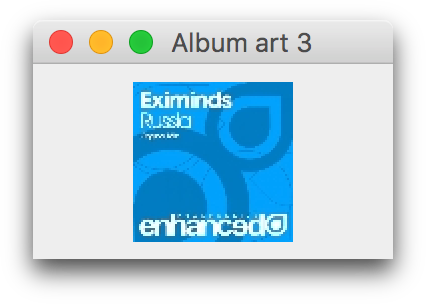
\includegraphics[width=4cm]{assets/Album-art-example}
  \caption{Example album art window}
  \label{fig:artworkExample}
\end{figure}

\subsection{Beat Grids}

The CDJs do not send any timing information other than beat numbers
during playback, which has made it difficult to offer absolute
timecode information. The discovery of beat grid requests provides a
clean answer to the problem. The beat grid for a track is a list of
every beat which occurs in the track, along with the point in time at
which that beat would occur if the track were played at its standard
(100\%) tempo. Armed with this table, it is possible to translate any
beat packet into an absolute position within the track, and, combined
with the tempo information, to generate timecode signals allowing
other software (such as video resources) to sync tightly with DJ
playback.

To request the beat grid of a track, send a message with $type$ {\tt
  0x2204} containing the $rekordbox$ ID of the track, like the one
shown in Figure~\ref{fig:beatGridRequest}.

\begin{figure}
  \begin{bytefield}[bitwidth=1.9em, leftcurly=., leftcurlyspace=0pt, boxformatting={\baselinealign}]{16}
    \hexhead \\
    \messagehead \\

    \begin{leftwordgroup}{\tiny\bfseries 00}

      \colorbitbox{lightgreen}{1}{\tt 11} & \colorbitbox{lightgreen}{4}{\tt 872349ae} &
      \colorbitbox{yellow}{1}{\tt 11} & \colorbitbox{yellow}{4}{$TxID$} &
      \colorbitbox{lightred}{1}{\tt 10} & \colorbitbox{lightred}{2}{\tt 2204} &
      \colorbitbox{lightcyan}{1}{\tt 0f} & \colorbitbox{lightcyan}{1}{\tt 02} &
      \colorbitbox{lightpurple}{1}{\tt 14}
    \end{leftwordgroup} \\

    \begin{leftwordgroup}{\tiny\bfseries 10}
      \colorbitbox{lightpurple}{4}{{\tt 0000000c}\small{ (12)}} &
      \colorbitbox[lbt]{lightpurple}{1}{\tt 06} & \colorbitbox[bt]{lightpurple}{1}{\tt 06} &
      \colorbitbox[bt]{lightpurple}{1}{\tt 00} & \colorbitbox[bt]{lightpurple}{1}{\tt 00} &
      \colorbitbox[bt]{lightpurple}{1}{\tt 00} & \colorbitbox[bt]{lightpurple}{1}{\tt 00} &
      \colorbitbox[bt]{lightpurple}{1}{\tt 00} & \colorbitbox[bt]{lightpurple}{1}{\tt 00} &
      \colorbitbox[bt]{lightpurple}{1}{\tt 00} & \colorbitbox[bt]{lightpurple}{1}{\tt 00} &
      \colorbitbox[bt]{lightpurple}{1}{\tt 00} & \colorbitbox[rbt]{lightpurple}{1}{\tt 00}
    \end{leftwordgroup} \\

    \begin{leftwordgroup}{\tiny\bfseries 20}
      \bitbox{1}{\tt 11} & \bitboxes*{1}{{$D$} {\tt 08} {$S_r$} {\tt 01}} &
      \bitbox{1}{\tt 11} & \bitbox{4}{$rekordbox$} & \bitbox[]{6}{}
    \end{leftwordgroup}

  \end{bytefield}
  \caption{Track beat grid request message}
  \label{fig:beatGridRequest}
\end{figure}

As usual, $seq$ should be incremented each time you send a query, and
will be used to identify the response messages. $D$ should have the
same value you used in your initial query context setup packet,
identifying the device that is asking the question. $S_r$ is the slot
in which the track being asked about can be found, and has the same
values used in CDJ status packets, as shown in
Figure~\ref{fig:cdjStatus}. Finally, $rekordbox$ identifies the
specific artwork image you are requesting, as found in a CDJ status
packet or playlist response. As with graphical requests, the value
after $D$, which identifies the location of the menu for which data is
being loaded, is 8.

The response will be a message with $type$ {\tt 0x4602}, containing
four arguments. The first argument echoes back our request type, which
was {\tt 0x2204}. The second always seems to be 0. The third contains
the length of the beat grid in bytes, which seems redundant, because
that is also conveyed in the fourth argument itself, which is a blob
containing the actual bytes of the beat grid, as shown in
Figure~\ref{fig:beatGridResponse}. However, if there is no beat grid
available, this value will be 0, and the blob field will be completely
omitted from the response, so you \emph{must not} try to read it!

\begin{figure}
  \begin{bytefield}[bitwidth=1.9em, leftcurly=., leftcurlyspace=0pt, boxformatting={\baselinealign}]{16}
    \hexhead \\
    \messagehead \\

    \begin{leftwordgroup}{\tiny\bfseries 00}

      \colorbitbox{lightgreen}{1}{\tt 11} & \colorbitbox{lightgreen}{4}{\tt 872349ae} &
      \colorbitbox{yellow}{1}{\tt 11} & \colorbitbox{yellow}{4}{$TxID$} &
      \colorbitbox{lightred}{1}{\tt 10} & \colorbitbox{lightred}{2}{\tt 4602} &
      \colorbitbox{lightcyan}{1}{\tt 0f} & \colorbitbox{lightcyan}{1}{\tt 04} &
      \colorbitbox{lightpurple}{1}{\tt 14}
    \end{leftwordgroup} \\

    \begin{leftwordgroup}{\tiny\bfseries 10}
      \colorbitbox{lightpurple}{4}{{\tt 0000000c}\small{ (12)}} &
      \colorbitbox[lbt]{lightpurple}{1}{\tt 06} & \colorbitbox[bt]{lightpurple}{1}{\tt 06} &
      \colorbitbox[bt]{lightpurple}{1}{\tt 06} & \colorbitbox[bt]{lightpurple}{1}{\tt 03} &
      \colorbitbox[bt]{lightpurple}{1}{\tt 00} & \colorbitbox[bt]{lightpurple}{1}{\tt 00} &
      \colorbitbox[bt]{lightpurple}{1}{\tt 00} & \colorbitbox[bt]{lightpurple}{1}{\tt 00} &
      \colorbitbox[bt]{lightpurple}{1}{\tt 00} & \colorbitbox[bt]{lightpurple}{1}{\tt 00} &
      \colorbitbox[bt]{lightpurple}{1}{\tt 00} & \colorbitbox[rbt]{lightpurple}{1}{\tt 00}
    \end{leftwordgroup} \\

    \begin{leftwordgroup}{\tiny\bfseries 20}
      \bitbox{1}{\tt 11} & \bitbox{4}{\tt 00002204} & \bitbox{1}{\tt 11} & \bitbox{4}{\tt 00000000} &
      \bitbox{1}{\tt 11} & \bitbox{4}{$length$} & \bitbox{1}{\tt 14}
    \end{leftwordgroup} \\

    \begin{leftwordgroup}{}
      \bitbox{4}{$length$} & \bitbox[lrt]{12}{Beat grid bytes} \\
      \skippedwords \\
      \wordbox[lrb]{1}{}
    \end{leftwordgroup}

  \end{bytefield}
  \caption{Track beat grid response message}
  \label{fig:beatGridResponse}
\end{figure}

The beat grid itself is spread through the value returned as argument
4, consisting of one-byte beat-within-bar numbers (labeled $B_b$ in
Figure~\ref{fig:cdjStatus}), followed by four-byte timing information,
specifying the number of milliseconds after the start of the track
(when played at its native tempo) at which that beat falls.

The $B_b$ value of the first beat in the track is found at byte 20 of
argument 4, and the time at which that beat occurs, in milliseconds,
is encoded as a 4-byte little-endian\footnote{Yes, unlike almost all
  numbers in the protocol, beat grid and cue point times are
  little-endian.} integer at bytes 21--24. Subsequent beats are found
at 16-byte intervals, so the second $B_b$ value is found at byte 36,
and the second beat's time, in milliseconds from the start of the
track, is the big-endian integer at bytes 37--40. The $B_b$ value for
the third beat is at byte 52, and its millisecond time is at bytes
53--56, and so on.

The purpose of the other bytes within the beat grid is so far
undetermined. It looks like there may be some sort of monotonically
increasing value following the beat millisecond value, but what it
means, and why it sometimes skips values, is mysterious.

\subsection{Requesting Track Waveforms}

Waveform data for tracks can be requested, both the preview, which is
400 pixels long, and the detailed waveform, which uses 150 pixels per
second of track content. (There is apparently another, more compact,
300 pixel preview format that Austin has seen, but since my players do
not use it, I don't know the request and response types for that.

To request the waveform preview of a track, send a message with $type$
{\tt 0x2004} containing the $rekordbox$ ID of the track, like the one
shown in Figure~\ref{fig:waveformPreviewRequest}.

\begin{figure}
  \begin{bytefield}[bitwidth=1.9em, leftcurly=., leftcurlyspace=0pt, boxformatting={\baselinealign}]{16}
    \hexhead \\
    \messagehead \\

    \begin{leftwordgroup}{\tiny\bfseries 00}

      \colorbitbox{lightgreen}{1}{\tt 11} & \colorbitbox{lightgreen}{4}{\tt 872349ae} &
      \colorbitbox{yellow}{1}{\tt 11} & \colorbitbox{yellow}{4}{$TxID$} &
      \colorbitbox{lightred}{1}{\tt 10} & \colorbitbox{lightred}{2}{\tt 2004} &
      \colorbitbox{lightcyan}{1}{\tt 0f} & \colorbitbox{lightcyan}{1}{\tt 05} &
      \colorbitbox{lightpurple}{1}{\tt 14}
    \end{leftwordgroup} \\

    \begin{leftwordgroup}{\tiny\bfseries 10}
      \colorbitbox{lightpurple}{4}{{\tt 0000000c}\small{ (12)}} &
      \colorbitbox[lbt]{lightpurple}{1}{\tt 06} & \colorbitbox[bt]{lightpurple}{1}{\tt 06} &
      \colorbitbox[bt]{lightpurple}{1}{\tt 06} & \colorbitbox[bt]{lightpurple}{1}{\tt 06} &
      \colorbitbox[bt]{lightpurple}{1}{\tt 03} & \colorbitbox[bt]{lightpurple}{1}{\tt 00} &
      \colorbitbox[bt]{lightpurple}{1}{\tt 00} & \colorbitbox[bt]{lightpurple}{1}{\tt 00} &
      \colorbitbox[bt]{lightpurple}{1}{\tt 00} & \colorbitbox[bt]{lightpurple}{1}{\tt 00} &
      \colorbitbox[bt]{lightpurple}{1}{\tt 00} & \colorbitbox[rbt]{lightpurple}{1}{\tt 00}
    \end{leftwordgroup} \\

    \begin{leftwordgroup}{\tiny\bfseries 20}
      \bitbox{1}{\tt 11} & \bitboxes*{1}{{$D$} {\tt 08} {$S_r$} {\tt 01}} &
      \bitbox{1}{\tt 11} & \bitbox{4}{\tt 00000004} &
      \bitbox{1}{\tt 11} & \bitbox{4}{$rekordbox$} & \bitbox{1}{\tt 11}
    \end{leftwordgroup} \\

    \begin{leftwordgroup}{\tiny\bfseries 30}
      \bitbox{4}{\tt 00000000} &
      \bitbox[]{12}{}
    \end{leftwordgroup}

  \end{bytefield}
  \caption{Waveform preview request message}
  \label{fig:waveformPreviewRequest}
\end{figure}

As usual, $seq$ should be incremented each time you send a query, and
will be used to identify the response messages. $D$ should have the
same value you used in your initial query context setup packet,
identifying the device that is asking the question. $S_r$ is the slot
in which the track being asked about can be found, and has the same
values used in CDJ status packets, as shown in
Figure~\ref{fig:cdjStatus}. Finally, $rekordbox$ identifies the
specific track whose waveform preview you are requesting, as found in
a CDJ status packet or playlist response. As with graphical requests,
the value after $D$, which identifies the location of the menu for
which data is being loaded, is 8.

You may have noticed that the argument list of the message in
Figure~\ref{fig:waveformPreviewRequest} specifies that there are five
arguments, but in fact the message contains only the first four,
numeric, arguments. The fifth, blob, argument is missing. This seems
to imply the blob is empty, and this very strange feature of the
protocol is, in fact, the way the track metadata is requested. The
fifth argument must be specified in the message header but not
actually present. When reading messages from a player, the same rules
apply: There is always a numeric field right before a blob field, and
it always contains a seemingly-redundant copy of the blob length, and
if that numeric field has the value $0$, you \emph{must not} try to
read the blob field. Instead, expect the next field or message to
follow the numeric field.

The second argument has an unknown purpose, but we have seen values of
3 or 4 for it. The fourth argument is the size of the blob argument we
are supposedly going to send; since we are not sending a blob, we
always send a 0 here.

The response will be a message with $type$ {\tt 0x4402}, containing
four arguments. The first argument echoes back our request type, which
was {\tt 0x2004}. The second always seems to be 0. The third contains
the length of the waveform preview in bytes. If this value is 0, the
fourth argument will be omitted from the response. When present, the
fourth argument is a blob containing the actual bytes of the waveform
preview, as shown in Figure~\ref{fig:waveformPreviewResponse}.

\begin{figure}
  \begin{bytefield}[bitwidth=1.9em, leftcurly=., leftcurlyspace=0pt, boxformatting={\baselinealign}]{16}
    \hexhead \\
    \messagehead \\

    \begin{leftwordgroup}{\tiny\bfseries 00}

      \colorbitbox{lightgreen}{1}{\tt 11} & \colorbitbox{lightgreen}{4}{\tt 872349ae} &
      \colorbitbox{yellow}{1}{\tt 11} & \colorbitbox{yellow}{4}{$TxID$} &
      \colorbitbox{lightred}{1}{\tt 10} & \colorbitbox{lightred}{2}{\tt 4402} &
      \colorbitbox{lightcyan}{1}{\tt 0f} & \colorbitbox{lightcyan}{1}{\tt 04} &
      \colorbitbox{lightpurple}{1}{\tt 14}
    \end{leftwordgroup} \\

    \begin{leftwordgroup}{\tiny\bfseries 10}
      \colorbitbox{lightpurple}{4}{{\tt 0000000c}\small{ (12)}} &
      \colorbitbox[lbt]{lightpurple}{1}{\tt 06} & \colorbitbox[bt]{lightpurple}{1}{\tt 06} &
      \colorbitbox[bt]{lightpurple}{1}{\tt 06} & \colorbitbox[bt]{lightpurple}{1}{\tt 03} &
      \colorbitbox[bt]{lightpurple}{1}{\tt 00} & \colorbitbox[bt]{lightpurple}{1}{\tt 00} &
      \colorbitbox[bt]{lightpurple}{1}{\tt 00} & \colorbitbox[bt]{lightpurple}{1}{\tt 00} &
      \colorbitbox[bt]{lightpurple}{1}{\tt 00} & \colorbitbox[bt]{lightpurple}{1}{\tt 00} &
      \colorbitbox[bt]{lightpurple}{1}{\tt 00} & \colorbitbox[rbt]{lightpurple}{1}{\tt 00}
    \end{leftwordgroup} \\

    \begin{leftwordgroup}{\tiny\bfseries 20}
      \bitbox{1}{\tt 11} & \bitbox{4}{\tt 00002004} & \bitbox{1}{\tt 11} & \bitbox{4}{\tt 00000000} &
      \bitbox{1}{\tt 11} & \bitbox{4}{$length$} & \bitbox{1}{\tt 14}
    \end{leftwordgroup} \\

    \begin{leftwordgroup}{}
      \bitbox{4}{$length$} & \bitbox[lrt]{12}{Waveform preview bytes} \\
      \skippedwords \\
      \wordbox[lrb]{1}{}
    \end{leftwordgroup}

  \end{bytefield}
  \caption{Waveform preview response message}
  \label{fig:waveformPreviewResponse}
\end{figure}

For this kind of waveform preview request,\footnote{There is an even
  lower-resolution preview available, with 4 bits of height per
  segment, and no shading, and there is also a full-color preview, but
  we don't yet know the requests needed to obtain these.} there are
900 bytes of waveform data returned. The first 800 of them contain 400
columns of waveform data, in the form of two-byte pairs, where the
first byte is the height of the waveform at that column (a value
ranging from 0 to 31), and the second byte is the whiteness, as
before, where 0 is blue and 7 is fully white. My players seem to only
pay attention to the highest bit of whiteness, drawing the waveform as
either very dark or light blue accordingly.

To experiment with this, start up dysentery in a Clojure REPL and
connect to a player as described in Section~\ref{sec:experimenting},
then evaluate an expression like {\tt (db/request-waveform-preview p2
  3 1060)}, replacing the arguments with the {\tt var} holding your
player connection, the proper $S_r$ number for the media slot the
track is found in, and the $rekordbox$ ID of the track, and dysentery
will open a window like Figure~{\ref{fig:waveformPreviewExample}}
showing the waveform preview.

\begin{figure}
  \vspace{5mm}
  \centering
  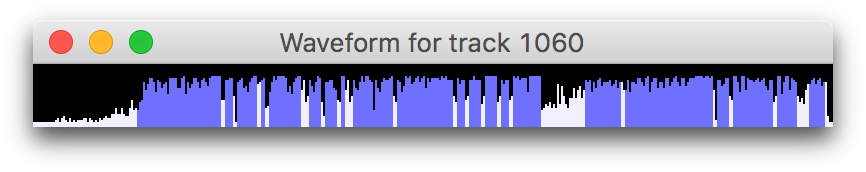
\includegraphics[width=8cm]{assets/Wave-preview-example}
  \caption{Example waveform preview window}
  \label{fig:waveformPreviewExample}
\end{figure}

I don't yet know what the remaining 100 bytes mean; perhaps they are
color information for players that support colored waveforms? More
likely, however, color uses a different request and response pair, and
we will have to wait for someone to take a packet capture of a nexus 2
player to see them.

Requesting the detailed waveform is very similar to requesting the
preview, but the request type and arguments are slightly different.
To request the detailed waveform of a track, send a message with $type$
{\tt 0x2904} containing the $rekordbox$ ID of the track, like the one
shown in Figure~\ref{fig:waveformDetailRequest}.

\begin{figure}
  \begin{bytefield}[bitwidth=1.9em, leftcurly=., leftcurlyspace=0pt, boxformatting={\baselinealign}]{16}
    \hexhead \\
    \messagehead \\

    \begin{leftwordgroup}{\tiny\bfseries 00}

      \colorbitbox{lightgreen}{1}{\tt 11} & \colorbitbox{lightgreen}{4}{\tt 872349ae} &
      \colorbitbox{yellow}{1}{\tt 11} & \colorbitbox{yellow}{4}{$TxID$} &
      \colorbitbox{lightred}{1}{\tt 10} & \colorbitbox{lightred}{2}{\tt 2904} &
      \colorbitbox{lightcyan}{1}{\tt 0f} & \colorbitbox{lightcyan}{1}{\tt 03} &
      \colorbitbox{lightpurple}{1}{\tt 14}
    \end{leftwordgroup} \\

    \begin{leftwordgroup}{\tiny\bfseries 10}
      \colorbitbox{lightpurple}{4}{{\tt 0000000c}\small{ (12)}} &
      \colorbitbox[lbt]{lightpurple}{1}{\tt 06} & \colorbitbox[bt]{lightpurple}{1}{\tt 06} &
      \colorbitbox[bt]{lightpurple}{1}{\tt 06} & \colorbitbox[bt]{lightpurple}{1}{\tt 00} &
      \colorbitbox[bt]{lightpurple}{1}{\tt 00} & \colorbitbox[bt]{lightpurple}{1}{\tt 00} &
      \colorbitbox[bt]{lightpurple}{1}{\tt 00} & \colorbitbox[bt]{lightpurple}{1}{\tt 00} &
      \colorbitbox[bt]{lightpurple}{1}{\tt 00} & \colorbitbox[bt]{lightpurple}{1}{\tt 00} &
      \colorbitbox[bt]{lightpurple}{1}{\tt 00} & \colorbitbox[rbt]{lightpurple}{1}{\tt 00}
    \end{leftwordgroup} \\

    \begin{leftwordgroup}{\tiny\bfseries 20}
      \bitbox{1}{\tt 11} & \bitboxes*{1}{{$D$} {\tt 01} {$S_r$} {\tt 01}} &
      \bitbox{1}{\tt 11} & \bitbox{4}{$rekordbox$} & \bitbox{1}{\tt 11} & \bitbox{4}{\tt 00000000} &
      \bitbox[]{1}{}
    \end{leftwordgroup} \\

  \end{bytefield}
  \caption{Waveform detail request message}
  \label{fig:waveformDetailRequest}
\end{figure}

As usual, $seq$ should be incremented each time you send a query, and
will be used to identify the response messages. $D$ should have the
same value you used in your initial query context setup packet,
identifying the device that is asking the question. $S_r$ is the slot
in which the track being asked about can be found, and has the same
values used in CDJ status packets, as shown in
Figure~\ref{fig:cdjStatus}. Finally, $rekordbox$ identifies the
specific track whose waveform preview you are requesting, as found in
a CDJ status packet or playlist response. Since this is a graphical
request, I would expect the value after $D$, which identifies the
location of the menu for which data is being loaded, to be 8 like it
is for others, but for some reason it is 1, which usually means the
main menu... maybe because the scrolling waveform appears in the same
location on the display as the main menu? In many ways this protocol
is a mystery wrapped in an enigma.

The waveform detail response is essentially identical to the waveform
preview response, with just the type numbers changed. It will be a
message with $type$ {\tt 0x4a02}, containing four arguments. The first
argument echoes back our request type, which was {\tt 0x2904}. The
second always seems to be 0. The third contains the length of the
waveform detail in bytes. If this value is 0, the fourth argument
will be omitted from the response. When present, the fourth argument
is a blob containing the actual bytes of the waveform detail, as
shown in Figure~\ref{fig:waveformDetailResponse}.

\begin{figure}
  \begin{bytefield}[bitwidth=1.9em, leftcurly=., leftcurlyspace=0pt, boxformatting={\baselinealign}]{16}
    \hexhead \\
    \messagehead \\

    \begin{leftwordgroup}{\tiny\bfseries 00}

      \colorbitbox{lightgreen}{1}{\tt 11} & \colorbitbox{lightgreen}{4}{\tt 872349ae} &
      \colorbitbox{yellow}{1}{\tt 11} & \colorbitbox{yellow}{4}{$TxID$} &
      \colorbitbox{lightred}{1}{\tt 10} & \colorbitbox{lightred}{2}{\tt 4a02} &
      \colorbitbox{lightcyan}{1}{\tt 0f} & \colorbitbox{lightcyan}{1}{\tt 04} &
      \colorbitbox{lightpurple}{1}{\tt 14}
    \end{leftwordgroup} \\

    \begin{leftwordgroup}{\tiny\bfseries 10}
      \colorbitbox{lightpurple}{4}{{\tt 0000000c}\small{ (12)}} &
      \colorbitbox[lbt]{lightpurple}{1}{\tt 06} & \colorbitbox[bt]{lightpurple}{1}{\tt 06} &
      \colorbitbox[bt]{lightpurple}{1}{\tt 06} & \colorbitbox[bt]{lightpurple}{1}{\tt 03} &
      \colorbitbox[bt]{lightpurple}{1}{\tt 00} & \colorbitbox[bt]{lightpurple}{1}{\tt 00} &
      \colorbitbox[bt]{lightpurple}{1}{\tt 00} & \colorbitbox[bt]{lightpurple}{1}{\tt 00} &
      \colorbitbox[bt]{lightpurple}{1}{\tt 00} & \colorbitbox[bt]{lightpurple}{1}{\tt 00} &
      \colorbitbox[bt]{lightpurple}{1}{\tt 00} & \colorbitbox[rbt]{lightpurple}{1}{\tt 00}
    \end{leftwordgroup} \\

    \begin{leftwordgroup}{\tiny\bfseries 20}
      \bitbox{1}{\tt 11} & \bitbox{4}{\tt 00002904} & \bitbox{1}{\tt 11} & \bitbox{4}{\tt 00000000} &
      \bitbox{1}{\tt 11} & \bitbox{4}{$length$} & \bitbox{1}{\tt 14}
    \end{leftwordgroup} \\

    \begin{leftwordgroup}{}
      \bitbox{4}{$length$} & \bitbox[lrt]{12}{Waveform detail bytes} \\
      \skippedwords \\
      \wordbox[lrb]{1}{}
    \end{leftwordgroup}

  \end{bytefield}
  \caption{Waveform detail response message}
  \label{fig:waveformDetailResponse}
\end{figure}

The content of the waveform detail is simpler and more compact than
the waveform preview. Every byte reperesents one segment of the
waveform, and there are 150 segments per second of audio. (These seem
to correspond to ``half frames'' counted as {\tt 03.5{\tiny F}} following the
seconds in the player display.) Each byte encodes both a color and
height. The three high-order bits encode the color, ranging from
darkest blue at 0 to near-white at 7. The five low-order bits encode
the height of the waveform at that point, from 0 to 31 pixels.

\subsection{Requesting Cue Points and Loops}

The locations of the cue points and loops stored in a track can be
obtained with a request like the one shown in
Figure~\ref{fig:cuePointRequestPacket}.

\begin{figure}
  \begin{bytefield}[bitwidth=1.9em, leftcurly=., leftcurlyspace=0pt, boxformatting={\baselinealign}]{16}
    \hexhead \\
    \messagehead \\

    \begin{leftwordgroup}{\tiny\bfseries 00}

      \colorbitbox{lightgreen}{1}{\tt 11} & \colorbitbox{lightgreen}{4}{\tt 872349ae} &
      \colorbitbox{yellow}{1}{\tt 11} & \colorbitbox{yellow}{4}{$TxID$} &
      \colorbitbox{lightred}{1}{\tt 10} & \colorbitbox{lightred}{2}{\tt 2104} &
      \colorbitbox{lightcyan}{1}{\tt 0f} & \colorbitbox{lightcyan}{1}{\tt 02} &
      \colorbitbox{lightpurple}{1}{\tt 14}
    \end{leftwordgroup} \\

    \begin{leftwordgroup}{\tiny\bfseries 10}
      \colorbitbox{lightpurple}{4}{{\tt 0000000c}\small{ (12)}} &
      \colorbitbox[lbt]{lightpurple}{1}{\tt 06} & \colorbitbox[bt]{lightpurple}{1}{\tt 06} &
      \colorbitbox[bt]{lightpurple}{1}{\tt 00} & \colorbitbox[bt]{lightpurple}{1}{\tt 00} &
      \colorbitbox[bt]{lightpurple}{1}{\tt 00} & \colorbitbox[bt]{lightpurple}{1}{\tt 00} &
      \colorbitbox[bt]{lightpurple}{1}{\tt 00} & \colorbitbox[bt]{lightpurple}{1}{\tt 00} &
      \colorbitbox[bt]{lightpurple}{1}{\tt 00} & \colorbitbox[bt]{lightpurple}{1}{\tt 00} &
      \colorbitbox[bt]{lightpurple}{1}{\tt 00} & \colorbitbox[rbt]{lightpurple}{1}{\tt 00}
    \end{leftwordgroup} \\

    \begin{leftwordgroup}{\tiny\bfseries 20}
      \bitbox{1}{\tt 11} & \bitboxes*{1}{{$D$} {\tt 08} {$S_r$} {\tt 01}} &
      \bitbox{1}{\tt 11} & \bitbox{4}{$rekordbox$} & \bitbox[]{6}{}
    \end{leftwordgroup}

  \end{bytefield}
  \caption{Cue point request message}
  \label{fig:cuePointRequestPacket}
\end{figure}

As always, $TxID$ should be 1 for the first query packet you send, 2
for the next, and so on. $D$ should have the same value you used in
your initial query context setup packet, identifying the device that
is asking the question. $S_r$ is the slot in which the track being
asked about can be found, and has the same values used in CDJ status
packets, as shown in Figure~\ref{fig:cdjStatus}, and as usual,
$rekordbox$ is the database ID of the track you're interested in.

The response will be a message with $type$ {\tt 0x4702}, containing
nine arguments. The first argument echoes back our request type, which
was {\tt 0x2104}. The second always seems to be 0. The third contains
the length of the blob containing cue and loop points in bytes, which
seems redundant, because that is also conveyed in the fourth argument
itself, which is a blob containing the actual bytes of the cue and
loop points, as shown in Figure~\ref{fig:cuePointResponse}.
However, if there are no cue or loop points, this value will be 0, and
the following blob field will be completely omitted from the response,
so you \emph{must not} try to read it!

The fifth argument is a number with uncertain purpose. It always seems
to have the value 36, which may be telling us the size of each
cue/loop point entry in argument 4 (they do seem to each take up 36
bytes, as shown in Figure~\ref{fig:cuePointEntry}). The sixth
argument, shown as $num_{hot}$, seems to contain the number of hot cue
entries found in argument 4, and the seventh, $num_{cue}$ seems to
contain the number of ordinary memory point cues. The eighth argument
is a number containing the length of the second binary field which
follows it. We don't know the meaning of the final, binary, argument.

\begin{figure}
  \begin{bytefield}[bitwidth=1.9em, leftcurly=., leftcurlyspace=0pt, boxformatting={\baselinealign}]{16}
    \hexhead \\
    \messagehead \\

    \begin{leftwordgroup}{\tiny\bfseries 00}

      \colorbitbox{lightgreen}{1}{\tt 11} & \colorbitbox{lightgreen}{4}{\tt 872349ae} &
      \colorbitbox{yellow}{1}{\tt 11} & \colorbitbox{yellow}{4}{$TxID$} &
      \colorbitbox{lightred}{1}{\tt 10} & \colorbitbox{lightred}{2}{\tt 4702} &
      \colorbitbox{lightcyan}{1}{\tt 0f} & \colorbitbox{lightcyan}{1}{\tt 09} &
      \colorbitbox{lightpurple}{1}{\tt 14}
    \end{leftwordgroup} \\

    \begin{leftwordgroup}{\tiny\bfseries 10}
      \colorbitbox{lightpurple}{4}{{\tt 0000000c}\small{ (12)}} &
      \colorbitbox[lbt]{lightpurple}{1}{\tt 06} & \colorbitbox[bt]{lightpurple}{1}{\tt 06} &
      \colorbitbox[bt]{lightpurple}{1}{\tt 06} & \colorbitbox[bt]{lightpurple}{1}{\tt 03} &
      \colorbitbox[bt]{lightpurple}{1}{\tt 06} & \colorbitbox[bt]{lightpurple}{1}{\tt 06} &
      \colorbitbox[bt]{lightpurple}{1}{\tt 06} & \colorbitbox[bt]{lightpurple}{1}{\tt 06} &
      \colorbitbox[bt]{lightpurple}{1}{\tt 03} & \colorbitbox[bt]{lightpurple}{1}{\tt 00} &
      \colorbitbox[bt]{lightpurple}{1}{\tt 00} & \colorbitbox[rbt]{lightpurple}{1}{\tt 00}
    \end{leftwordgroup} \\

    \begin{leftwordgroup}{\tiny\bfseries 20}
      \bitbox{1}{\tt 11} & \bitbox{4}{\tt 00002104} & \bitbox{1}{\tt 11} & \bitbox{4}{\tt 00000000} &
      \bitbox{1}{\tt 11} & \bitbox{4}{$length_1$} & \bitbox{1}{\tt 14}
    \end{leftwordgroup} \\

    \begin{leftwordgroup}{}
      \bitbox{4}{$length_1$} & \bitbox[lrt]{12}{Cue and loop point bytes} \\
      \skippedwords \\
      \bitbox[lrb]{1}{} & \bitbox{1}{\tt 11} & \bitbox{4}{{\tt 00000036}} &
      \bitbox{1}{\tt 11} & \bitbox{4}{$num_{hot}$} & \bitbox{1}{\tt 11} & \bitbox{4}{$num_{cue}$} \\
      \bitbox{1}{\tt 11} & \bitbox{4}{$length_2$} &
      \bitbox{1}{\tt 14} & \bitbox{4}{$length_2$} &\bitbox[lrt]{6}{Unknown bytes} \\
      \skippedwords \\
      \wordbox[lrb]{1}{}
    \end{leftwordgroup}

  \end{bytefield}
  \caption{Cue point response message}
  \label{fig:cuePointResponse}
\end{figure}

As described above, the first binary field in the cue point response
is divided up in to 36 byte entries, each of which potentially holds a
cue or loop point. They are not in any particular order, with respect
to the time at which they occur in the track. They each have the
structure shown in Figure~\ref{fig:cuePointEntry}.

The first byte, $F_l$, has the value $1$ if this entry specifies a
loop, or $0$ otherwise. The second byte, $F_c$, has the value $1$ if
this entry contains a cue point, and $0$ otherwise. Entries with loops
have the value $1$ in both of these bytes, because loops also act as
cue points. If both values are $0$, the entry is ignored (it is
probably a leftover cue point that was deleted by the DJ). The third
byte, labeled $H$, is $0$ for ordinary cue points, but has a value if
this entry defines a hot cue. Hot cues A through C are represented by
the values $1$, $2$, and $3$.

The actual location of the cue and loop points are in the values $cue$
and $loop$. These are both 4-byte integers, and like beat grid
positions, but unlike essentially every other number in the protocol,
they are stored with a little-endian byte order. For non-looping cue
points, only $cue$ has a meaning, and it identifies the position of
the cue point in the track, in \( \frac{1}{150} \) second units. For
loops, $cue$ identifies the start of the loop, and $loop$ identifies
the end of the loop, again in \( \frac{1}{150} \) second units.

\begin{figure}
  \begin{bytefield}[bitwidth=1.9em, leftcurly=., leftcurlyspace=0pt, boxformatting={\baselinealign}]{16}
    \hexhead \\

    \begin{leftwordgroup}{\tiny\bfseries 00}
      \bitbox{1}{$F_l$} & \bitbox{1}{$F_c$} & \bitbox{1}{$H$} &
      \bitboxes*{1}{{\tt 00} {\tt 00} {\tt 00} {\tt 00} {\tt 00} {\tt 00} {\tt 00} {\tt 00} {\tt 00}} &
      \bitbox{4}{$cue$}
    \end{leftwordgroup} \\

    \begin{leftwordgroup}{\tiny\bfseries 10}
      \bitbox{4}{$loop$} &
      \bitboxes*{1}{{\tt 00} {\tt 00} {\tt 00} {\tt 00} {\tt 00} {\tt 00}
        {\tt 00} {\tt 00} {\tt 00} {\tt 00} {\tt 00} {\tt 00}}
    \end{leftwordgroup} \\

    \begin{leftwordgroup}{\tiny\bfseries 20}
      \bitboxes*{1}{{\tt 00} {\tt 00} {\tt 00} {\tt 00}} & \bitbox[]{12}{}
    \end{leftwordgroup} \\

  \end{bytefield}
  \caption{Cue/loop point entry}
  \label{fig:cuePointEntry}
\end{figure}






\subsection{Requesting All Tracks}
\label{sec:allTracks}

If you want to cache all the metadata associated with a media stick,
this query is a good starting point. Send a packet like the
one shown in Figure~\ref{fig:trackListSetupPacket}.

\begin{figure}
  \begin{bytefield}[bitwidth=1.9em, leftcurly=., leftcurlyspace=0pt, boxformatting={\baselinealign}]{16}
    \hexhead \\
    \messagehead \\

    \begin{leftwordgroup}{\tiny\bfseries 00}

      \colorbitbox{lightgreen}{1}{\tt 11} & \colorbitbox{lightgreen}{4}{\tt 872349ae} &
      \colorbitbox{yellow}{1}{\tt 11} & \colorbitbox{yellow}{4}{$TxID$} &
      \colorbitbox{lightred}{1}{\tt 10} & \colorbitbox{lightred}{2}{\tt 1004} &
      \colorbitbox{lightcyan}{1}{\tt 0f} & \colorbitbox{lightcyan}{1}{\tt 02} &
      \colorbitbox{lightpurple}{1}{\tt 14}
    \end{leftwordgroup} \\

    \begin{leftwordgroup}{\tiny\bfseries 10}
      \colorbitbox{lightpurple}{4}{{\tt 0000000c}\small{ (12)}} &
      \colorbitbox[lbt]{lightpurple}{1}{\tt 06} & \colorbitbox[bt]{lightpurple}{1}{\tt 06} &
      \colorbitbox[bt]{lightpurple}{1}{\tt 00} & \colorbitbox[bt]{lightpurple}{1}{\tt 00} &
      \colorbitbox[bt]{lightpurple}{1}{\tt 00} & \colorbitbox[bt]{lightpurple}{1}{\tt 00} &
      \colorbitbox[bt]{lightpurple}{1}{\tt 00} & \colorbitbox[bt]{lightpurple}{1}{\tt 00} &
      \colorbitbox[bt]{lightpurple}{1}{\tt 00} & \colorbitbox[bt]{lightpurple}{1}{\tt 00} &
      \colorbitbox[bt]{lightpurple}{1}{\tt 00} & \colorbitbox[rbt]{lightpurple}{1}{\tt 00}
    \end{leftwordgroup} \\

    \begin{leftwordgroup}{\tiny\bfseries 20}
      \bitbox{1}{\tt 11} & \bitboxes*{1}{{$D$} {\tt 01} {$S_r$} {\tt 01}} &
      \bitbox{1}{\tt 11} & \bitbox{4}{$sort$} & \bitbox[]{6}{}
    \end{leftwordgroup}

  \end{bytefield}
  \caption{Full track list request message}
  \label{fig:trackListSetupPacket}
\end{figure}

As always, $TxID$ should be 1 for the first query packet you send, 2
for the next, and so on. $D$ should have the same value you used in
your initial query context setup packet, identifying the device that
is asking the question. $S_r$ is the slot in which the track being
asked about can be found, and has the same values used in CDJ status
packets, as shown in Figure~\ref{fig:cdjStatus}. The new $sort$
parameter determines the order in which the tracks are sorted, and
that also affects the item type returned, along with the secondary
information (beyond the title) that it contains about the track, as
described in Section~\ref{sec:trackListSorting}. We will start out
assuming the tracks are being requested in title order, which can be
done by sending a $sort$ argument value of 0 or 1.

Track list requests (just like metadata requests) are built on the
mechanism that is used to request and draw scrollable menus on the
CDJs. The player responds with a success indicator, saying it is ready
to send these ``menu items'' and reporting how many of them are
available, much like shown in Figure~\ref{fig:trackSetupResponse},
although the first argument will be {\tt 0x1004} to reflect the
message type we just sent, rather than {\tt 0x2002} as it was for the
metadata request.

As with metadata, the next step is to send a ``render menu'' request
like that in Figure~\ref{fig:renderMenuRequest} to get the actual
results. But the number of results available is likely to be much
higher than shown in Figure~\ref{fig:trackSetupResponse}, because we
have asked about all tracks in the media slot. That means we will
probably need more than one ``render menu'' request to get them all.

I don't know how many items you can safely ask for at one time. I have
had success with values as high as 64 on my CDJ-2000 nexus players,
but they failed when asking for numbers in the thousands. So to be
safe, you should ask for the results in chunks of 64 or smaller, by
setting $limit$ and $limit2$ to the smaller of 64 and the remaining
number of results you want, and incrementing $offset$ by 64 in each
request until you have retrieved them all.

As with metadata requests, you will get back two more messages than
you ask for, because you first get a menu header message (with $type$
{\tt 0x4001}, Figure~\ref{fig:trackMetadataMenuHeader}), then the
requested menu items are sent (with $type$ {\tt 0x4101},
Figure~\ref{fig:trackMetadataMenuItem}), and finally these are
followed by a menu footer message (with $type$ {\tt 0x4201},
Figure~\ref{fig:trackMetadataMenuFooter}). This wrapping happens with
all ``render menu'' requests, and the menu footer is an easy way to
know you are done, although you can also count the messages.

The details of the menu items are slightly different than in the case
of a metadata request. In the example where you are retrieving tracks
in title order, they will have content like this:

\begin{center}
  \begin{tabu}{rcX}
    \toprule

    \bfseries{Arg} & \bfseries{Type} & \bfseries{Meaning} \\

    1 & number & artist id \\

    2 & number & $rekordbox$ id of track \\

    3 & number & length in bytes of Label 1 \\

    4 & string & Label 1, Track Title \\

    5 & number & length in bytes of Label 2 \\

    6 & string & Label 2, Artist Name \\

    7 & number & type of this item, {\tt 0x704} for this sort order \\

    8 & number & some sort of flags field, details still unclear \\

    9 & number & unknown \\

    10 & number & unknown \\

    11 & number & unknown \\

    12 & number & unknown \\

    \bottomrule
  \end{tabu}
\end{center}

\subsubsection{Alternate Track List Sort Orders}
\label{sec:trackListSorting}

As noted above, you can request the track list in a diferent order by
supplying a different value for the $sort$ parameter. The value 0 or 1
gives the order and information just described. The $sort$ values
discovered so far are shown in the following table, and return menu
items with the specified type values in argument 7.

\begin{center}
  \begin{tabu}{rcX}
    \toprule

    \bfseries{Sort} & \bfseries{Type} & \bfseries{Description} \\

    1 & {\tt 0x704} & Sorted by track title, described above \\

    2 & {\tt 0x704} & Sorted by artist name, same item type \\

    3 & {\tt 0x204} & Sorted by album, Arg 1 becomes album ID, Label 2 becomes album name \\

    4 & {\tt 0xd04} & Sorted by BPM, Arg 1 becomes BPM$\times$100, Label 2 empty \\

    6 & {\tt 0x604} & Sorted by genre, Arg 1 becomes genre ID, Label 2 becomes genre name \\

    7 & {\tt 0x2304} & Sorted by comment, Label 2 becomes comment \\

    \bottomrule
  \end{tabu}
\end{center}

To experiment with this, start up dysentery in a Clojure REPL and
connect to a player as described in Section~\ref{sec:experimenting},
then evaluate an expression like {\tt (db/request-track-list p2 3)},
replacing the arguments with the {\tt var} holding your player
connection and the proper $S_r$ number for the media slot containing
the tracks you want to list. You can also add a third argument to
specify a sort order, like this to sort all the tracks in the USB slot
by BPM:

{\tt (db/request-track-list p2 3 4)}


\subsection{Playlists}

If you want to be more selective about the metadata that you are
caching, you can navigate the playlist folder hierarchy and deal with
only specific playlists. This process is essentially the same as asking
for all tracks, except that in the playlist request you specify the
playlist or folder that you want to list. To start at the root of the
playlist folder hierarchy, you request folder 0. A playlist request
has the struture shown in Figure~\ref{fig:playlistSetupPacket}.

\begin{figure}
  \begin{bytefield}[bitwidth=1.9em, leftcurly=., leftcurlyspace=0pt, boxformatting={\baselinealign}]{16}
    \hexhead \\
    \messagehead \\

    \begin{leftwordgroup}{\tiny\bfseries 00}

      \colorbitbox{lightgreen}{1}{\tt 11} & \colorbitbox{lightgreen}{4}{\tt 872349ae} &
      \colorbitbox{yellow}{1}{\tt 11} & \colorbitbox{yellow}{4}{$TxID$} &
      \colorbitbox{lightred}{1}{\tt 10} & \colorbitbox{lightred}{2}{\tt 1105} &
      \colorbitbox{lightcyan}{1}{\tt 0f} & \colorbitbox{lightcyan}{1}{\tt 04} &
      \colorbitbox{lightpurple}{1}{\tt 14}
    \end{leftwordgroup} \\

    \begin{leftwordgroup}{\tiny\bfseries 10}
      \colorbitbox{lightpurple}{4}{{\tt 0000000c}\small{ (12)}} &
      \colorbitbox[lbt]{lightpurple}{1}{\tt 06} & \colorbitbox[bt]{lightpurple}{1}{\tt 06} &
      \colorbitbox[bt]{lightpurple}{1}{\tt 06} & \colorbitbox[bt]{lightpurple}{1}{\tt 06} &
      \colorbitbox[bt]{lightpurple}{1}{\tt 00} & \colorbitbox[bt]{lightpurple}{1}{\tt 00} &
      \colorbitbox[bt]{lightpurple}{1}{\tt 00} & \colorbitbox[bt]{lightpurple}{1}{\tt 00} &
      \colorbitbox[bt]{lightpurple}{1}{\tt 00} & \colorbitbox[bt]{lightpurple}{1}{\tt 00} &
      \colorbitbox[bt]{lightpurple}{1}{\tt 00} & \colorbitbox[rbt]{lightpurple}{1}{\tt 00}
    \end{leftwordgroup} \\

    \begin{leftwordgroup}{\tiny\bfseries 20}
      \bitbox{1}{\tt 11} & \bitboxes*{1}{{$D$} {\tt 01} {$S_r$} {\tt 01}} &
      \bitbox{1}{\tt 11} & \bitbox{4}{$sort$} & \bitbox{1}{\tt 11} & \bitbox{4}{$id$} & \bitbox{1}{\tt 11}
    \end{leftwordgroup} \\

    \begin{leftwordgroup}{\tiny\bfseries 30}
      \bitbox{4}{$folder?$} & \bitbox[]{12}{}
    \end{leftwordgroup}

  \end{bytefield}
  \caption{Playlist request message}
  \label{fig:playlistSetupPacket}
\end{figure}

As always, $TxID$ should be 1 for the first query packet you send, 2
for the next, and so on. $D$ should have the same value you used in
your initial query context setup packet, identifying the device that
is asking the question. $S_r$ is the slot in which the track being
asked about can be found, and has the same values used in CDJ status
packets, as shown in Figure~\ref{fig:cdjStatus}. You specify the ID of
the playlist or folder you want to list in the $id$ argument, and set
$folder?$ to 1 if you are asking for a folder, and 0 if you are asking
for a playlist. As noted above, to get the top-level list of
playlists, ask for folder 0, by passing an $id$ of 0 and passing
$folder?$ as 1.

Much as when listing all tracks, the response may tell you there are
more entries in the playlist than you can retreive in a single
request, so you should follow the procedure outlined in
Section~\ref{sec:allTracks} to request your results in smaller
batches. The followup queries that you send are identical for
playlists as they are described in that section. The actual menu items
returned when you are asking for a folder have the following content:

\begin{center}
  \begin{tabu}{rcX}
    \toprule

    \bfseries{Arg} & \bfseries{Type} & \bfseries{Meaning} \\

    1 & number & parent folder id \\

    2 & number & id of playlist or folder \\

    3 & number & length in bytes of Label 1 \\

    4 & string & Label 1, Name of playlist or folder \\

    5 & number & length in bytes of Label 2 \\

    6 & string & Label 2, empty \\

    7 & number & type of this item, {\tt 0x1} for folder, {\tt 0x8} for playlist \\

    8 & number & unknown \\

    9 & number & unknown \\

    10 & number & playlist position \\

    11 & number & unknown \\

    12 & number & unknown \\

    \bottomrule
  \end{tabu}
\end{center}

When you have requested a playlist (by passing its $id$ and a value of
0 for $folder?$) the responses you get are track list entries, just
like when you request all tracks as shown in
Section~\ref{sec:allTracks}. And just like in that section, you can
get the results in a different order by specifying a value for $sort$.
The supported values and corresponding item types returned seem to be
the same as described there. Additionally, if you pass a $sort$ value
of 9, the playlist entries will come back sorted by track title, Label
2 will be empty, and the item type will be {\tt 0x2904}.

To experiment with this, start up dysentery in a Clojure REPL and
connect to a player as described in Section~\ref{sec:experimenting},
then evaluate an expression like {\tt (db/request-playlist p2 3 1)},
replacing the arguments with the {\tt var} holding your player
connection, the proper $S_r$ number for the media slot containing the
playlist you want to list, and the playlist ID. You can also add a
third argument to specify that you want to list a folder, like this
using folder ID 0 to request the root folder:

{\tt (db/request-playlist p2 3 0 true)}

Finally, you can add a fourth argument to specify a sort order, like
this to sort all the tracks in playlist 12 by genre:

{\tt (db/request-playlist p2 3 12 false 6)}

\subsection{Experimenting with Metadata}
\label{sec:experimenting}

The best way to get a feel for the details of working with these
messages is to load dysentery into a Clojure REPL, as described on the
project page, and play with some of the functions in the {\tt
  dysentery.dbserver} namespace. Have no more than three players
connected and active on your network, so you have an unused player
number for dysentery to use. In this example, player number 1 is
available, so we set dysentery up to pose as player 1:

\begin{footnotesize}\begin{alltt}
> \textbf{lein repl}
nREPL server started on port 53806 on host 127.0.0.1 -
 nrepl://127.0.0.1:53806
REPL-y 0.3.7, nREPL 0.2.12
Clojure 1.8.0
Java HotSpot(TM) 64-Bit Server VM 1.8.0_77-b03
dysentery loaded.
dysentery.core=> \textbf{(view/watch-devices :player-number 1)}
Looking for DJ Link devices...
Found:
   DJM-2000nexus 33 /172.16.42.3
   CDJ-2000nexus 2 /172.16.42.4

To communicate create a virtual CDJ with address
  /172.16.42.2, MAC address 3c:15:c2:e7:08:6c,
  and use broadcast address /172.16.42.255
{:socket #object[java.net.DatagramSocket 0x22b952b1
                 "java.net.DatagramSocket@22b952b1"],
 :watcher #future[{:status :pending, :val nil} 0x3eb8f41b]}
dysentery.core> \textbf{(def p2 (db/connect-to-player 2 1))}
Transaction: 4294967294, message type: 0x4000
 (requested data available), argument count: 2, arguments:
  number:          0 (0x00000000) [request type]
  number:          2 (0x00000002) [# items available]
#'dysentery.core/p2
dysentery.core> \textbf{(def md (db/request-metadata p2 2 1))}
Sending > Transaction: 1, message type: 0x2002
 (request track metadata), argument count: 2, arguments:
  number:   16843265 (0x01010201) [player, menu, media, 1]
  number:          1 (0x00000001) [rekordbox ID]
Received > Transaction: 1, message type: 0x4000
 (requested data available), argument count: 2, arguments:
  number:       8194 (0x00002002) [request type]
  number:         11 (0x0000000b) [# items available]
Sending > Transaction: 2, message type: 0x3000
 (render menu), argument count: 6, arguments:
  number:   16843265 (0x01010201) [player, menu, media, 1]
  number:          0 (0x00000000) [offset]
  number:         11 (0x0000000b) [limit]
  number:          0 (0x00000000) [unknown (0)?]
  number:         11 (0x0000000b) [len_a (= limit)?]
  number:          0 (0x00000000) [unknown (0)?]
Received 1  > Transaction: 2, message type: 0x4001
 (rendered menu header), argument count: 2, arguments:
  number:          1 (0x00000001) [unknown]
  number:          0 (0x00000000) [unknown]
Received 2  > Transaction: 2, message type: 0x4101
 (rendered menu item), argument count: 12, arguments:
  number:          1 (0x00000001) [numeric 1 (parent id)]
  number:          1 (0x00000001) [numeric 2 (this id)]
  number:         80 (0x00000050) [label 1 byte size]
  string: "Escape ft. Zoë Phillips" [label 1]
  number:          2 (0x00000002) [label 2 byte size]
  string: "" [label 2]
  number:          4 (0x00000004) [item type: Track Title]
  number:   16777216 (0x01000000) [column configuration?]
  number:          0 (0x00000000) [album art id]
  number:          0 (0x00000000) [playlist position]
  number:        256 (0x00000100) [unknown]
  number:          0 (0x00000000) [unknown]
...
Received 13  > Transaction: 2, message type: 0x4201
 (rendered menu footer), argument count: 0, arguments:
#'dysentery.core/md
dysentery.core>
\end{alltt}\end{footnotesize}

In this interaction, after setting up the watcher so we can find
players on the network, we set the {\tt var} p2 to be a connection to
player 2, in which we are posing as player 1. Then we submit a
metadata request to {\tt p2}, requesting the track in slot 2 (SD
card), with $rekordbox$ id 1. You can see the messages being sent and
received to accomplish that. For more functions that you can call,
including the very flexible {\tt experiment} function, look at the
source for the {\tt dysentery.dbserver} namespace. Most of the
response messages containing track metadata were omitted for brevity;
you will get more meaningful results trying it with your own tracks,
and then you can see all the details.

\section{What's Missing?}

We know this analysis isn't complete. Here are some loose ends to
explore.

\subsection{Background Research}

Prior to Evan and Austin's breakthroughs, here is all we knew:

By setting up a managed switch to mirror traffic sent directly between
CDJs, we have been able to see how the Link Info operation is
implemented: The players open a direct TCP connection between each
other, and send queries to obtain the metadata about tracks with
particular rekordbox ID values.

Using an Ethernet switch
with port mirroring was, as we hoped, very helpful. As can be seen in
the capture at
\url{https://github.com/brunchboy/dysentery/raw/master/doc/assets/LinkInfo.pcapng},
which shows a CDJ with IP address 169.254.192.112 booting, the new CDJ
opens two TCP connections to the other CDJ at 169.254.119.181.

The first session (given id 0 by Wireshark), which begins at packet
206, connecting to port 12523, determines the port to use for metadata
queries.

The second TCP connection (Wireshark display filter {\tt tcp.stream eq
  1}), beginning at packet 212 and connecting to port 1051, shows the
track information used by the Link Info display passing between the
CDJs. You can see packets reflecting the initial display of a track
that was already loaded, then new information as the linked CDJ loaded
three other tracks.

There is another capture at
\url{https://github.com/brunchboy/dysentery/raw/master/doc/assets/LinkInfo2.pcapng},
with more Link Info streams to be studied (all of the odd numbered
{\tt tcp.stream} values in Wireshark are the relevant ones).

\subsection{Deeper Emulation and Tempo Mastery}

With the help of Austin's {\tt
 libpdjl}\footnote{\url{https://bitbucket.org/awwright/libpdjl}}, it
looks like it will be possible to emulate a CDJ well enough to act as
a tempo master, which will allow bidirectional sync with Ableton Link.
This is probably my next area of focus.

It should also be easy enough to capture the traffic that rekordbox
sends when it tells a player to load and start playing a track, and
reproduce that.

\subsection{Mysterious Values}

There are still many values with unknown meanings described above, and
many menu types that have yet to be explored; I hav focused on the
ones that will be immediately useful to Beat Link Trigger.
Contributions of additional research and insight are eagerly
welcomed---I would have not gotten nearly this far without help!

\subsection{Reading Data Without a CDJ}

In order to offer metadata, timecode, waveforms, and so on, when there
are four actual CDJs on the network, it is necessary to pre-load and
cache all the data, since dbserver queries are not possible with all
player numbers in use. While this can be done with a single CDJ
powered up, it would be really nice to be able to read the information
right out of the rekordbox files on the media that the DJ will be
using for the show. So far, we don't know how to do that.

Before we discovered how to ask players for metadata about
particular tracks, we did some research into the underlying rexordbox
database. The database format is called
DeviceSQL,\footnote{\url{https://www.quora.com/What-database-system-did-Greg-Kemnitz-develop}}
and there used to be a free quick start suite for working with
it\footnote{\url{http://java.sys-con.com/node/328557}} but that site
no longer exists because the original (California) company
Encirq\footnote{\url{https://www.crunchbase.com/organization/encirq-corporation}}
was acquired by the Japanese Ubiquitous Corporation in
2008.\footnote{\url{http://www.ubiquitous.co.jp/en/news/press/pdf/p1730_01.pdf}}
It seems to still be
available,\footnote{\url{http://www.ubiquitous.co.jp/en/products/db/md/devicesql/}}
but I'd be surprised if they wanted to help out an open source effort
like this one.

It looks like, other than the textual metadata in the {\tt .edb} file,
the format of the files containing the other crucial information (beat
grid, wave forms, cue lists) is figured
out,\footnote{\url{https://reverseengineering.stackexchange.com/questions/4311/help-reversing-a-edb-database-file-for-pioneers-rekordbox-software}}
so a possible half-measure would be to create a half-baked metadata
cache file whose track titles are based on the file paths, and which
contains everything but the other text information, and then provide a
mechanism for combining that with queries for just the text metadata
to build a complete cache much more quickly at the start of a show.

\subsection{CDJ Packets to Rekordbox}

Performing a packet capture while rekordbox is running reveals that
the CDJs send unicast packets to the rekordbox address on port 50000,
in addition to the packets they normally broadcast on that port.
Figuring out how to pose as rekordbox might be useful in order to see
what additional data these can offer, although that may be much more
work than posing as a CDJ.

\subsection{Dysentery}

If you have access to Pioneer equipment and are willing to help us
validate this analysis, and perhaps even figure out more details, you
can find the tool that is being used to perform this research at: \\
\url{https://github.com/brunchboy/dysentery}

\begin{appendix}

  \listoffigures

  \begin{center}
    \begin{samepage}
      
\includegraphics[width=4cm]{assets/DS-Logo-bw-4k}

      \vspace{0.25cm}
      \url{http://deepsymmetry.org}
    \end{samepage}
  \end{center}

\end{appendix}

\end{document}

